\documentclass[10pt,a4paper]{article}

% --- LANGUAGE AND ENCODING ---
\usepackage{iftex}
\ifPDFTeX
  \usepackage[utf8]{inputenc}
  \usepackage[T5,T1]{fontenc}
  \usepackage[vietnamese]{babel}
  \usepackage{lmodern}
\else
  \usepackage{fontspec}
  \setmainfont{Times New Roman}
\fi

% --- PAGE LAYOUT & GEOMETRY ---
\usepackage[a4paper, top=20mm, bottom=22mm, left=20mm, right=20mm, footskip=12mm]{geometry}
\usepackage{fancyhdr}
\pagestyle{fancy}
\fancyhf{}
\renewcommand{\headrulewidth}{0.4pt}
\fancyhead[L]{\small\textit{Báo cáo Kiến trúc Mô hình RAPT-CLIP \& Thực nghiệm}}
\fancyhead[R]{\small\textit{RAPT-CLIP Research}}
\fancyfoot[C]{\small Trang \thepage}

% --- MATH & SYMBOLS ---
\usepackage{amsmath,amssymb,amsfonts,bm}

% --- GRAPHICS & FLOATS ---
\usepackage{graphicx}
\usepackage{subcaption}
\usepackage{float}
\usepackage{caption}
\captionsetup{font=small, labelfont=bf, skip=5pt}

% --- TABLES & COLORS ---
\usepackage{booktabs}
\usepackage{tabularx}
\usepackage{multirow}
\usepackage{array}
\usepackage[table,xcdraw]{xcolor}
\definecolor{primaryblue}{RGB}{24, 76, 120}
\definecolor{tableheader}{RGB}{240, 243, 246}
\definecolor{grouprow}{RGB}{232, 238, 245}
\definecolor{codebg}{RGB}{248, 250, 252}
\definecolor{codeborder}{RGB}{59, 130, 246}
\definecolor{accentgreen}{RGB}{34, 139, 34}
\definecolor{accentred}{RGB}{198, 40, 40}

% --- CODE LISTINGS & BOXES ---
\usepackage{listings}
\usepackage{tcolorbox}
\tcbuselibrary{skins,breakable}

\lstset{
  language=Python,
  basicstyle=\ttfamily\scriptsize,
  keywordstyle=\color{primaryblue}\bfseries,
  stringstyle=\color{teal},
  commentstyle=\color{gray}\itshape,
  numbers=none,
  breaklines=true,
  breakatwhitespace=true,
  tabsize=4,
  showstringspaces=false
}

% --- HYPERLINKS ---
\usepackage{hyperref}
\hypersetup{
    colorlinks=true,
    linkcolor=primaryblue,
    citecolor=primaryblue,
    urlcolor=blue
}

% --- SECTION FORMATTING ---
\usepackage{titlesec}
\titleformat{\section}{\color{primaryblue}\normalfont\large\bfseries}{\thesection.}{0.8em}{}[\titlerule]
\titleformat{\subsection}{\normalfont\normalsize\bfseries}{\thesubsection}{0.6em}{}
\titleformat{\subsubsection}{\normalfont\small\bfseries}{\thesubsubsection}{0.5em}{}
\titlespacing*{\section}{0pt}{14pt}{8pt}
\titlespacing*{\subsection}{0pt}{10pt}{5pt}
\titlespacing*{\subsubsection}{0pt}{8pt}{4pt}

% --- DOCUMENT INFO ---
\title{\vspace{-10mm}\Huge\bfseries\color{primaryblue} Báo Cáo Chi Tiết\\Kiến Trúc Mô Hình RAPT-CLIP và Thực Nghiệm}
\author{\textbf{Nhóm Nghiên Cứu RAPT-CLIP} \\ Khoa Khoa học \& Kỹ thuật Máy tính}
\date{\today}

\begin{document}

\maketitle
\thispagestyle{fancy}

\begin{abstract}
\noindent Báo cáo trình bày chi tiết kiến trúc mô hình \textbf{RAPT-CLIP} (Robust Attention Prompt Tuning CLIP) cho bài toán nhận diện cảm xúc và sự tập trung học tập đa phương thức. Báo cáo phân tích chuyên sâu cơ chế dung hợp chú ý chéo đa phương thức ở cấp độ khung hình (\textit{Frame-Level Cross-Modal Attention Fusion - CMAF}), nhánh thích ứng biểu cảm khuôn mặt (\textit{Face Adapter - EAA}), và mô hình hóa thời gian thống nhất (\textit{Unified Temporal Transformer}). Đồng thời, tài liệu đối chiếu toàn diện các kết quả thực nghiệm, tính bền vững (\textit{Robustness}), giải thích mô hình (\textit{Grad-CAM}), các nghiên cứu cắt bỏ thành phần (\textit{Ablation Studies}) trên bộ dữ liệu \textbf{RAER}, cùng kết quả đánh giá đa nhãn SOTA và siêu tham số chi tiết trên bộ dữ liệu \textbf{EMOTIC}, \textbf{CAER} và \textbf{DAiSEE}.
\end{abstract}

\vspace{2mm}

% ==============================================================================
% MỤC 1: TỔNG QUAN MÔ HÌNH
% ==============================================================================
\section{Tổng quan mô hình}

\subsection{So sánh kiến trúc tổng thể}

\begin{figure}[H]
    \centering
    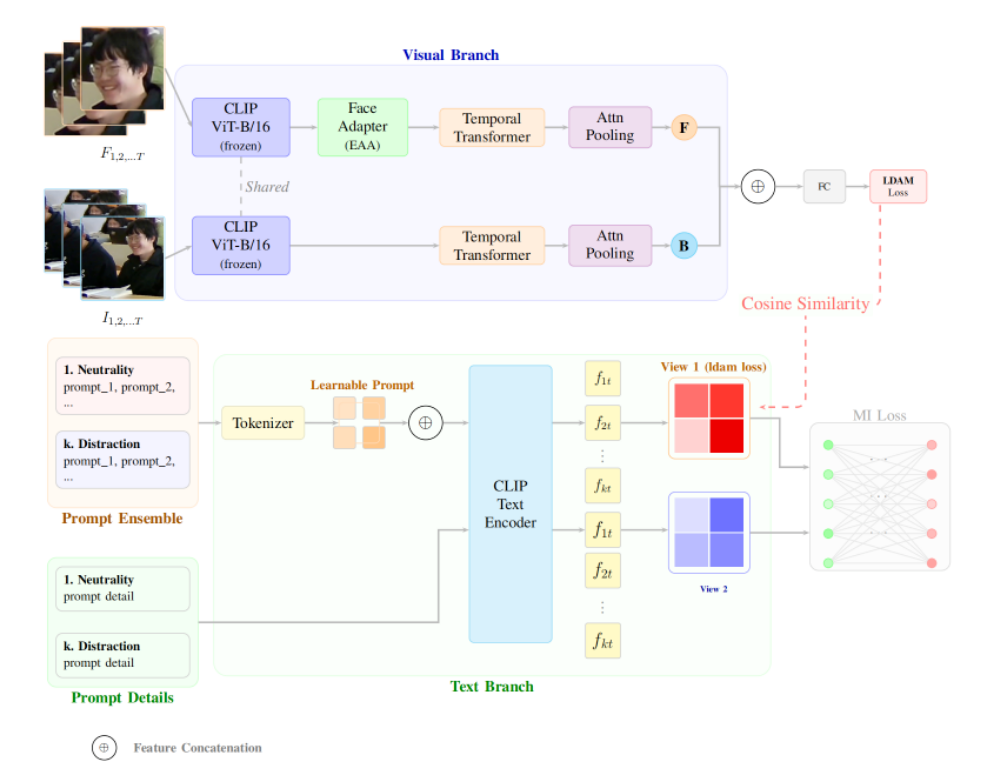
\includegraphics[width=0.88\textwidth, max height=7cm, keepaspectratio]{image/old_model.png}
    \caption{Kiến trúc mô hình RAPT-CLIP cũ (\textit{Video-Level Fusion})}
    \label{fig:old_model}
\end{figure}

\begin{figure}[H]
    \centering
    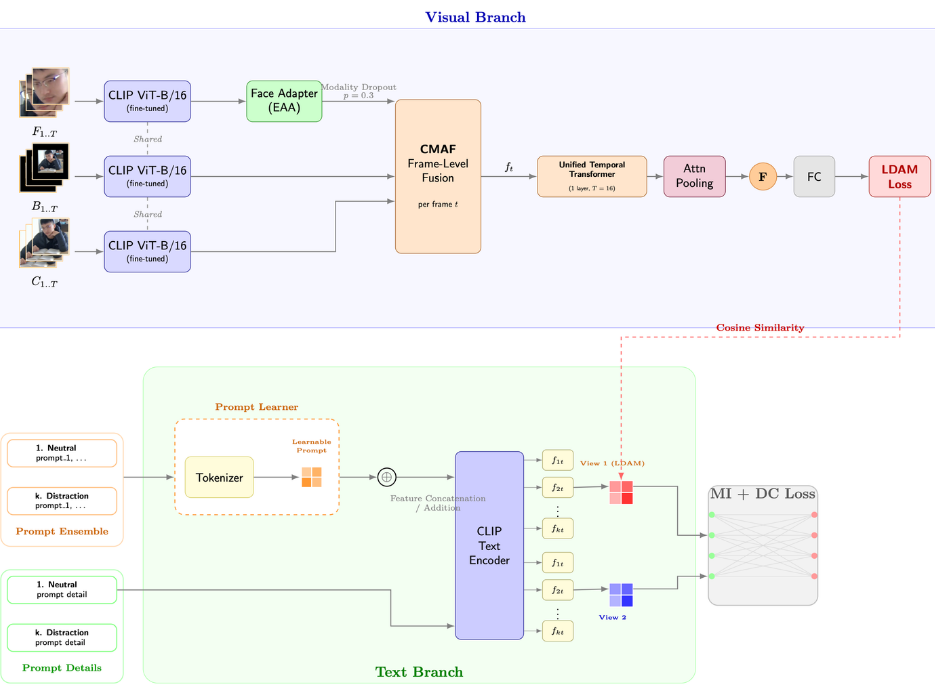
\includegraphics[width=0.92\textwidth, max height=7.5cm, keepaspectratio]{image/model.png}
    \caption{Tổng quan kiến trúc mô hình RAPT-CLIP mới đề xuất (\textit{Frame-Level CMAF})}
    \label{fig:new_model}
\end{figure}

\noindent\textbf{So sánh cốt lõi:} Mô hình cũ sử dụng cơ chế \textit{Video-Level Fusion}: mỗi luồng trong ba luồng (Khuôn mặt - Face, Thân trên - Body, Toàn cảnh bối cảnh - Context) tự nén qua một mạng Temporal riêng biệt trước khi ghép nối ở mức video. Cách làm này khiến tương tác ngữ cảnh giữa các phương thái bị trễ và thiếu liên kết vi mô tại từng thời điểm. Ngược lại, mô hình mới đề xuất áp dụng cơ chế \textit{Frame-Level CMAF}: ba luồng tương tác chéo với nhau ngay tại từng khung hình $t$, trao đổi và làm giàu ngữ cảnh trước khi ghép nối (\textit{Concat}) và đưa qua một mạng \textbf{Unified Temporal Transformer} duy nhất. Cơ chế mới vừa tăng cường độ nhạy bén cảm xúc, vừa giảm 50\% số lượng tham số mạng thời gian.

% ------------------------------------------------------------------------------
\subsection{Nhánh hình ảnh}

\subsubsection{Face Adapter (EAA)}
Xét ví dụ trực quan về một học sinh trong video lớp học đang có dấu hiệu ngủ gật:
\begin{itemize}[leftmargin=18pt, itemsep=1pt]
    \item \textbf{Face (512 chiều):} Hai mắt nhắm nghiền. Tuy nhiên, nếu chỉ nhìn khuôn mặt, hệ thống rất dễ nhầm lẫn giữa chớp mắt thông thường và ngủ gật thực sự.
    \item \textbf{Body (512 chiều):} Đầu gục xuống mặt bàn, hai vai buông thõng, lưng còng.
    \item \textbf{Context (512 chiều):} Không gian bàn học trong lớp, ánh sáng phòng học, sách vở xung quanh.
\end{itemize}

Khối \textbf{Expression-Aware Adapter (EAA)} được tích hợp trực tiếp vào nhánh khuôn mặt với cấu trúc mạng thắt nút cổ chai (\textit{Bottleneck MLP}: $512 \rightarrow 128 \rightarrow 512$) kết hợp kết nối tàn dư (\textit{Residual Connection}). Khối EAA giúp bộ mã hóa thị giác CLIP ViT-B/16 nhạy bén hơn với các đơn vị vận động vi mô trên cơ mặt (\textit{Action Units} như nhắm mắt, nhăn trán, trễ môi) mà không làm biến dạng các trọng số tiền huấn luyện tổng quát ban đầu của CLIP.

% ------------------------------------------------------------------------------
\subsubsection{Khối Cross-Modal Attention Fusion (CMAF) \& Phép Concat}
Khối CMAF đóng vai trò trung tâm trong việc quyết định độ chính xác cảm xúc. Bảng~\ref{tab:cmaf_io} đặc tả chi tiết các luồng tensor đầu vào, đầu ra trung gian và đầu ra cuối cùng của hệ thống.

\begin{table}[H]
\centering
\small
\caption{Bảng đặc tả chi tiết Tensor Đầu vào và Đầu ra của khối CMAF}
\label{tab:cmaf_io}
\begin{tabularx}{\textwidth}{p{2.6cm} p{2.2cm} p{3.2cm} X}
\toprule
\rowcolor{tableheader}
\textbf{Tên Tensor} & \textbf{Kích thước} & \textbf{Nguồn gốc / Đích đến} & \textbf{Ý nghĩa nghiệp vụ} \\
\midrule
\rowcolor{grouprow} \multicolumn{4}{l}{\textbf{I. Đầu vào (Inputs của khối CMAF)}} \\
\texttt{face\_feat} & $(B, 512)$ & CLIP ViT-B/16 + EAA & Đặc trưng biểu cảm mặt vi mô tại từng khung hình. \\
\texttt{body\_feat} & $(B, 512)$ & CLIP ViT-B/16 (Upper-body) & Đặc trưng tư thế cơ thể (đầu gục, vai thả lỏng). \\
\texttt{context\_feat} & $(B, 512)$ & CLIP ViT-B/16 (Full Image) & Đặc trưng bối cảnh không gian lớp học, ánh sáng. \\
\midrule
\rowcolor{grouprow} \multicolumn{4}{l}{\textbf{II. Đầu ra trung gian (Sau Cross-Attention)}} \\
\texttt{face\_out} & $(B, 512)$ & Mặt sau khi hỏi Thân + Cảnh & Khuôn mặt đã được làm giàu ngữ cảnh (hiểu mắt nhắm do ngủ). \\
\texttt{body\_out} & $(B, 512)$ & Thân sau khi hỏi Mặt + Cảnh & Tư thế cơ thể được giải nghĩa dựa trên biểu cảm mặt. \\
\texttt{context\_out} & $(B, 512)$ & Cảnh sau khi hỏi Mặt + Thân & Bối cảnh được lọc sạch nhiễu nền, tập trung chủ thể. \\
\midrule
\rowcolor{grouprow} \multicolumn{4}{l}{\textbf{III. Đầu ra cuối cùng (Sau Concatenation \& Pipeline)}} \\
\texttt{fused\_frame} & $(B, 1536)$ & Ghép 3 luồng ($512 \times 3$) & Vector hợp nhất đa phương thức đầy đủ tại từng frame. \\
\texttt{video\_features} & $(N, 512)$ & Sau Temporal + Projection & Vector đại diện video chuẩn hóa $L_2$ để tính Cosine Similarity. \\
\bottomrule
\end{tabularx}
\vspace{1mm}
\raggedright\footnotesize\textit{* Ghi chú: Kích thước batch ở cấp độ khung hình là $B = N \times 16$ ($N$ là batch size video, 16 là số khung hình lấy mẫu).}
\end{table}

\noindent\textbf{Chi tiết 5 bước vận hành của cơ chế CMAF \& Concat:}
\begin{enumerate}[leftmargin=18pt, itemsep=2pt]
    \item \textbf{Tạo Tokens Truy vấn (Query) và Khóa/Giá trị (Key/Value):} Mỗi luồng đóng vai trò là một token Query: $\bm{Q} = \text{feat}.\text{unsqueeze}(1) \in \mathbb{R}^{B \times 1 \times 512}$. Hai luồng còn lại được ghép nối thành chuỗi Key và Value gồm 2 tokens: $\bm{K} = \bm{V} = \text{cat}([\dots], \text{dim}=1) \in \mathbb{R}^{B \times 2 \times 512}$.
    \item \textbf{Cơ chế tương tác chéo tam hướng (Cross-Attention với 4 Heads):} Chiếu tuyến tính sang 4 đầu chú ý ($d_k = 128$). Tính tích vô hướng chuẩn hóa và Softmax để xác định trọng số tương quan chéo:
    \begin{equation}
        \text{Attention\_Weights} = \text{Softmax}\left(\frac{\bm{Q}\bm{K}^T}{\sqrt{128}}\right) = [\alpha_{\text{luồng\_1}}, \alpha_{\text{luồng\_2}}]
    \end{equation}
    Ví dụ: Khi khuôn mặt có mắt nhắm, mạng tự động gán trọng số chú ý cao vào tư thế gục đầu của thân để khẳng định trạng thái ngủ gật.
    \item \textbf{Cộng tàn dư (Residual) và Chuẩn hóa lớp (LayerNorm):} Vector sau chú ý được cộng trực tiếp với vector đặc trưng gốc của luồng đó nhằm bảo toàn thông tin bản thể, sau đó đi qua LayerNorm để ổn định phân phối gradient:
    \begin{equation}
        \text{out} = \text{LayerNorm}(\text{CrossAttn} + \text{feat}) \in \mathbb{R}^{B \times 512}
    \end{equation}
    \item \textbf{Phép nối tiếp Concat (Tại sao dùng Concat thay vì Add?):} Lệnh \texttt{torch.cat((face\_out, body\_out, context\_out), dim=-1)} ghép ba vector 512 chiều thành vector \textbf{1536 chiều}. Phép cộng (\textit{Add}) sẽ triệt tiêu các đặc trưng vi mô riêng biệt (Action Units của mặt bị lấn át bởi màu sắc nền). Phép nối (\textit{Concat}) bảo toàn nguyên vẹn cả ba không gian biểu diễn độc lập để các tầng sâu hơn tự học cách trích lọc tổ hợp phi tuyến tính tối ưu.
    \item \textbf{Dòng dữ liệu sau Concat:} Tensor $(B, 1536)$ được chuyển về dạng chuỗi video $(N, 16, 1536) \rightarrow$ đưa qua \textit{Unified Temporal Transformer} để nắm bắt tiến trình thời gian $\rightarrow$ nén qua \textit{Attention Pooling} thành $(N, 1536) \rightarrow$ chiếu qua \textit{Linear Projection Head} về $(N, 512)$ và chuẩn hóa $L_2$ để tính tích vô hướng Cosine Similarity với Text Embeddings.
\end{enumerate}

\begin{tcolorbox}[
    enhanced,
    colback=codebg,
    colframe=codeborder,
    boxrule=1pt,
    leftrule=3.5pt,
    arc=2mm,
    title={\small\textbf{Mã nguồn PyTorch hoàn chỉnh: Cơ chế CMAF \& Luồng xử lý Forward}},
    coltitle=white,
    colbacktitle=primaryblue,
    breakable
]
\begin{lstlisting}
import torch
import torch.nn as nn

class CrossModalAttentionFusion(nn.Module):
    def __init__(self, dim=512, num_heads=4, dropout=0.1, use_context=True):
        super().__init__()
        self.use_context = use_context
        # 3 khoi MultiheadAttention tam huong (dim=512, 4 heads -> dim_head=128)
        self.cross_attn_f2bc = nn.MultiheadAttention(dim, num_heads, dropout=dropout, batch_first=True)
        self.norm_f          = nn.LayerNorm(dim)

        self.cross_attn_b2fc = nn.MultiheadAttention(dim, num_heads, dropout=dropout, batch_first=True)
        self.norm_b          = nn.LayerNorm(dim)

        self.cross_attn_c2fb = nn.MultiheadAttention(dim, num_heads, dropout=dropout, batch_first=True)
        self.norm_c          = nn.LayerNorm(dim)

    def forward(self, face_feat, body_feat, context_feat):
        # BUOC 1: TIEP NHAN DAU VAO (face_feat, body_feat, context_feat: B x 512)
        
        # BUOC 2: CROSS-ATTENTION VOI QUERY = 1 token, KEY/VALUE = 2 tokens
        # 2.1 Mat hoi (Query) Than & Canh:
        face_q          = face_feat.unsqueeze(1)                                                 # (B, 1, 512)
        body_context_kv = torch.cat((body_feat.unsqueeze(1), context_feat.unsqueeze(1)), dim=1) # (B, 2, 512)
        face_cross, _   = self.cross_attn_f2bc(query=face_q, key=body_context_kv, value=body_context_kv)
        face_out        = self.norm_f(face_cross.squeeze(1) + face_feat)                         # (B, 512)

        # 2.2 Than hoi (Query) Mat & Canh:
        body_q          = body_feat.unsqueeze(1)                                                 # (B, 1, 512)
        face_context_kv = torch.cat((face_feat.unsqueeze(1), context_feat.unsqueeze(1)), dim=1) # (B, 2, 512)
        body_cross, _   = self.cross_attn_b2fc(query=body_q, key=face_context_kv, value=face_context_kv)
        body_out        = self.norm_b(body_cross.squeeze(1) + body_feat)                         # (B, 512)

        # 2.3 Canh hoi (Query) Mat & Than:
        context_q       = context_feat.unsqueeze(1)                                              # (B, 1, 512)
        face_body_kv    = torch.cat((face_feat.unsqueeze(1), body_feat.unsqueeze(1)), dim=1)    # (B, 2, 512)
        context_cross, _ = self.cross_attn_c2fb(query=context_q, key=face_body_kv, value=face_body_kv)
        context_out     = self.norm_c(context_cross.squeeze(1) + context_feat)                   # (B, 512)

        # BUOC 3: CONCATENATION DOC THEO CHIEU DAC TRUNG (dim=-1)
        fused_frame_features = torch.cat((face_out, body_out, context_out), dim=-1)             # (B, 1536)
        return fused_frame_features

# ==============================================================================
# PIPELINE XU LY TIEP THEO TRONG GenerateModel (models/Generate_Model.py):
# 1. Reshape ve chuoi video: fused_seq = fused_frame_features.view(N, 16, 1536)
# 2. Qua Unified Temporal Transformer & Pooling: video_features = self.temporal_net(fused_seq) # (N, 1536)
# 3. Chieu ve 512-d & chuan hoa L2: video_features = F.normalize(self.project_fc(video_features), p=2, dim=-1)
# 4. Tinh Cosine Similarity: logits = (video_features @ text_features.T) / self.temperature
# ==============================================================================
\end{lstlisting}
\end{tcolorbox}

% ------------------------------------------------------------------------------
\subsubsection{Unified Temporal Transformer}
Sau khi ghép nối tại từng khung hình tạo thành chuỗi 16 vector 1536 chiều, toàn bộ chuỗi được đưa vào một mạng \textbf{Unified Temporal Transformer} duy nhất. Khối này học được quỹ đạo biến đổi cảm xúc theo thời gian (ví dụ: chuyển từ tập trung sang ngáp ngủ), đồng thời tiết kiệm 50\% bộ nhớ tham số so với việc triển khai ba mạng Temporal độc lập như cấu trúc cũ.

% ==============================================================================
% MỤC 2: HUẤN LUYỆN TRÊN RAER
% ==============================================================================
\section{Huấn luyện trên bộ dữ liệu RAER}

\noindent\textbf{Đường dẫn Kaggle:} \href{https://www.kaggle.com/code/bearmn/vision-learning-academic-emotion-understanding}{Kaggle Notebook - Vision Learning Academic Emotion Understanding (v4)}

\subsection{Bảng đối chiếu siêu tham số huấn luyện chi tiết}
Bảng~\ref{tab:raer_hyperparams} đối chiếu toàn bộ cấu hình giữa mô hình tối ưu \texttt{RAPT-CLIP-FRAMELEVELFUSION} và mô hình so sánh \texttt{RAPT-CLIP-VIDEOLEVELFUSION}.

\begin{table}[H]
\centering
\small
\caption{Bảng đối chiếu siêu tham số huấn luyện trên bộ dữ liệu RAER}
\label{tab:raer_hyperparams}
\begin{tabularx}{\textwidth}{p{3.8cm} X X}
\toprule
\rowcolor{tableheader}
\textbf{Tham số (Flag)} & \textbf{RAPT-CLIP-FRAMELEVELFUSION} & \textbf{RAPT-CLIP-VIDEOLEVELFUSION} \\
\midrule
\rowcolor{grouprow} \multicolumn{3}{l}{\textbf{1. Cấu hình kiến trúc \& Dung hợp}} \\
\texttt{--fusion-stage} & \textbf{frame} (CMAF frame $\rightarrow$ Unified Temporal) & \textbf{video} (Temporal từng luồng $\rightarrow$ Concat muộn) \\
\texttt{--fusion-type} & \texttt{cmaf} & \texttt{cmaf} \\
\texttt{--temporal-layers} & 1 (Unified Transformer) & 1 (3 Temporal Transformers độc lập) \\
\texttt{--use-context} & True (Face + Body + Context) & True (Face + Body + Context) \\
\texttt{--crop-body} & True (Cắt nửa thân trên 70\%) & True (Cắt nửa thân trên 70\%) \\
\texttt{--modality-dropout} & 0.3 & 0.3 \\
\midrule
\rowcolor{grouprow} \multicolumn{3}{l}{\textbf{2. Cấu hình dữ liệu \& Thị giác}} \\
\texttt{--dataset} & RAER & RAER \\
\texttt{--clip-path} & ViT-B/16 (OpenAI CLIP) & ViT-B/16 (OpenAI CLIP) \\
\texttt{--num-segments} & 16 khung hình / video & 16 khung hình / video \\
\texttt{--image-size} & $224 \times 224$ & $224 \times 224$ \\
\texttt{--batch-size} / \texttt{--epochs} & 2 / 20 epochs & 2 / 20 epochs \\
\texttt{--seed} / \texttt{--use-amp} & 42 / True (Mixed Precision) & 42 / True (Mixed Precision) \\
\midrule
\rowcolor{grouprow} \multicolumn{3}{l}{\textbf{3. Tối ưu hóa \& Learning Rate}} \\
\texttt{--optimizer} / \texttt{--weight-decay} & AdamW / 0.005 & AdamW / 0.005 \\
\texttt{--lr} (Temporal/FC) & $2\times 10^{-5}$ & $2\times 10^{-5}$ \\
\texttt{--lr-image-encoder} & $1\times 10^{-6}$ & $1\times 10^{-6}$ \\
\texttt{--lr-prompt-learner} & $3\times 10^{-4}$ & $3\times 10^{-4}$ \\
\texttt{--lr-adapter} & $1\times 10^{-4}$ & $1\times 10^{-4}$ \\
\texttt{--scheduler} / \texttt{--milestones} & MultiStepLR / [10, 15] ($\gamma = 0.1$) & MultiStepLR / [10, 15] ($\gamma = 0.1$) \\
\midrule
\rowcolor{grouprow} \multicolumn{3}{l}{\textbf{4. Hàm mất mát \& Cân bằng nhãn}} \\
\texttt{--loss-type} & LDAM & LDAM \\
\texttt{--ldam-s} / \texttt{--ldam-max-m} & 30.0 / 0.5 & 30.0 / 0.5 \\
\texttt{--label-smoothing} & 0.05 & 0.05 \\
\texttt{--use-weighted-sampler} & True & True \\
\texttt{--lambda\_mi} / \texttt{--lambda\_dc} & 0.1 / 0.1 (warmup 5, ramp 10) & 0.1 / 0.1 (warmup 5, ramp 10) \\
\texttt{--text-type} / \texttt{contexts-number} & prompt\_ensemble / 8 tokens & prompt\_ensemble / 8 tokens \\
\bottomrule
\end{tabularx}
\end{table}

\subsection{Kết quả thực nghiệm trên RAER}

\begin{figure}[H]
    \centering
    \begin{subfigure}[b]{0.48\textwidth}
        \centering
        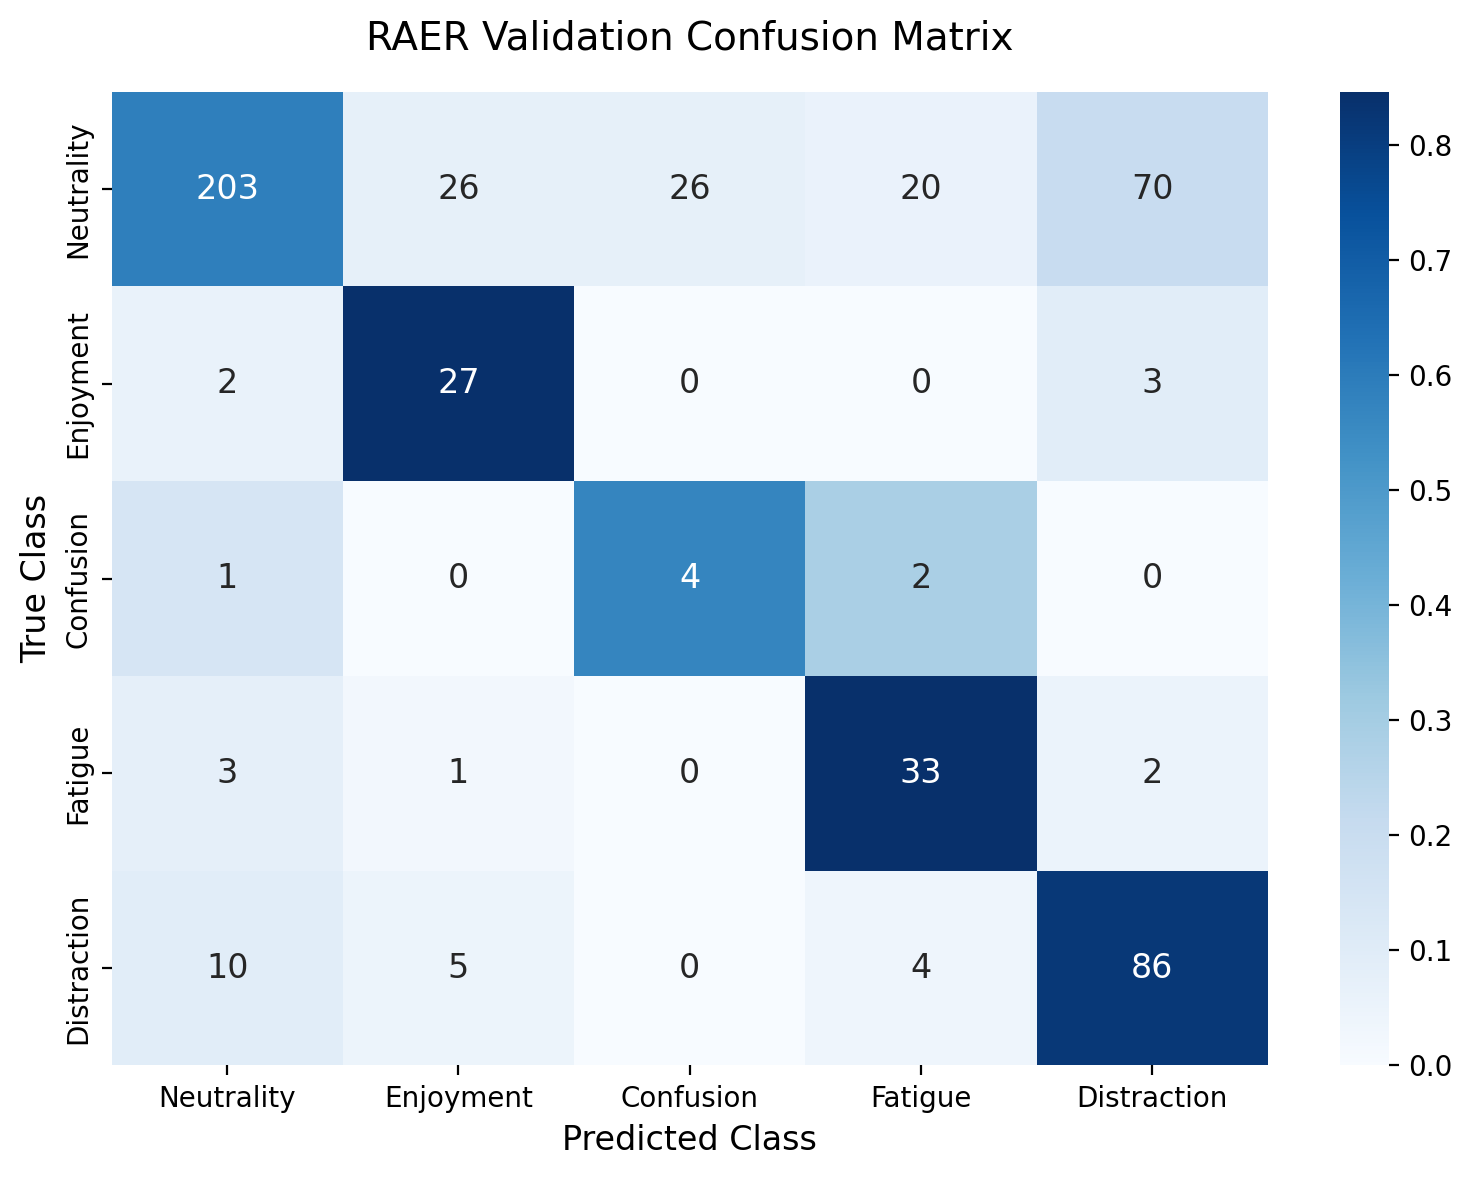
\includegraphics[width=\textwidth]{image/confusion_matrix.png}
        \caption{Ma trận nhầm lẫn (Confusion Matrix)}
        \label{fig:raer_cm}
    \end{subfigure}
    \hfill
    \begin{subfigure}[b]{0.48\textwidth}
        \centering
        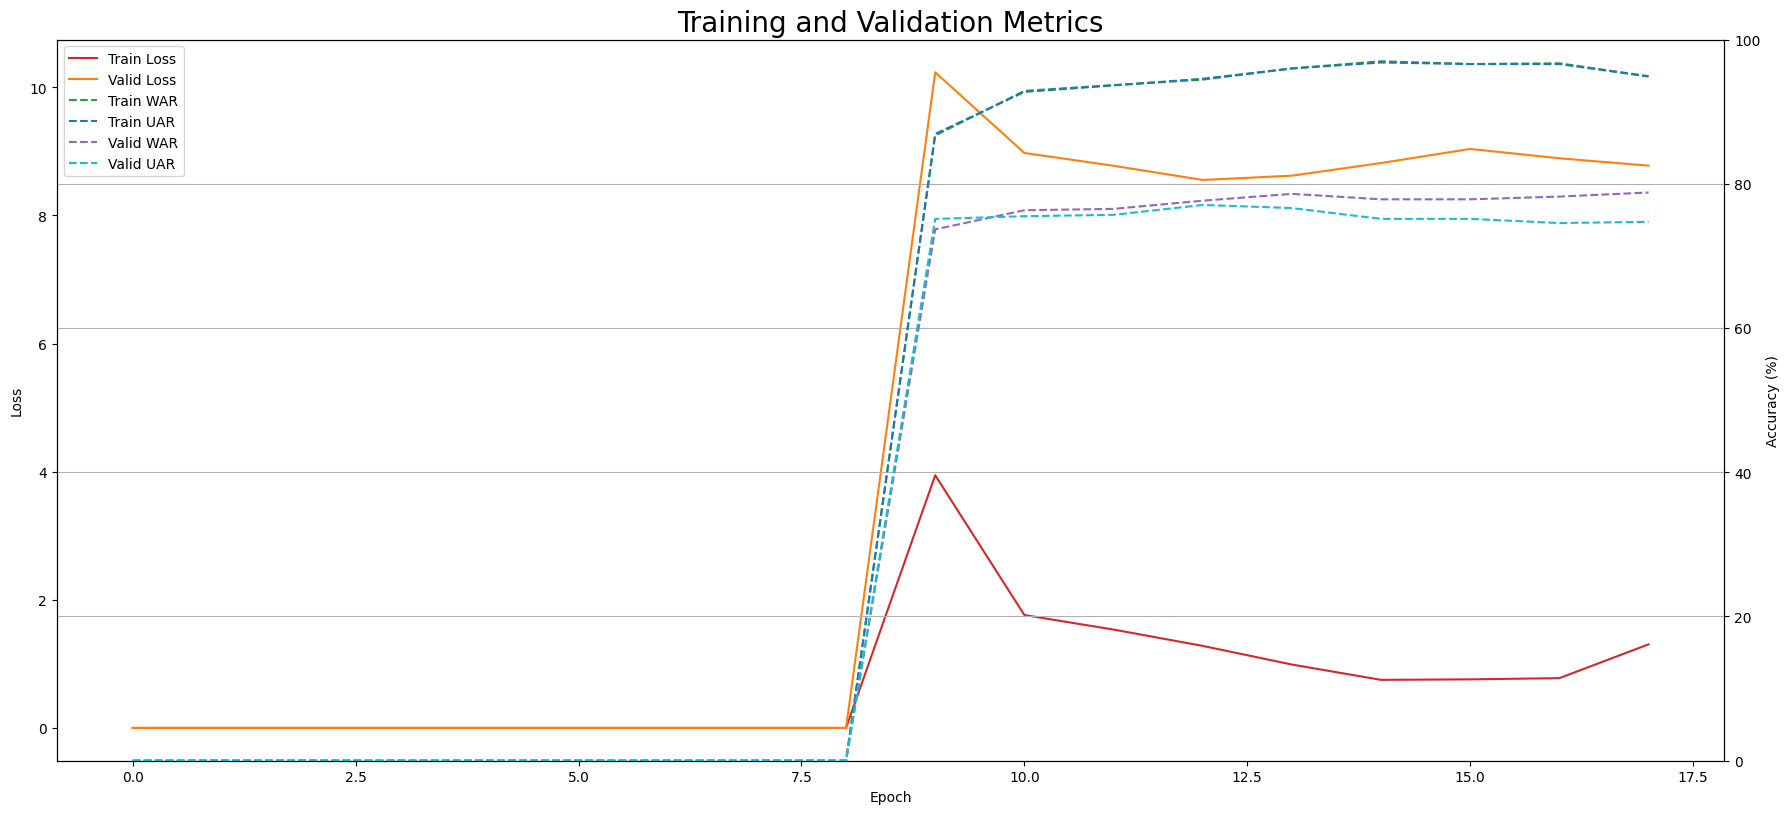
\includegraphics[width=\textwidth]{image/training_curves.png}
        \caption{Đường cong huấn luyện (Training Curves)}
        \label{fig:raer_curves}
    \end{subfigure}
    \caption{Kết quả đánh giá trên tập kiểm thử RAER (WAR: 77.65\%, UAR: 77.06\%)}
    \label{fig:raer_results}
\end{figure}

\subsection{Trực quan hóa t-SNE \& Các đánh giá thực nghiệm chuyên sâu}

\subsubsection{Không gian đặc trưng t-SNE (Pretrained CLIP vs Fine-tuned RAPT-CLIP)}
Thuật toán t-SNE giảm chiều không gian vector đặc trưng 512 chiều xuống 2 chiều trên toàn bộ 528 video tập kiểm thử RAER (5 lớp cảm xúc: Neutrality, Enjoyment, Confusion, Fatigue, Distraction).

\begin{figure}[H]
    \centering
    \begin{subfigure}[b]{0.48\textwidth}
        \centering
        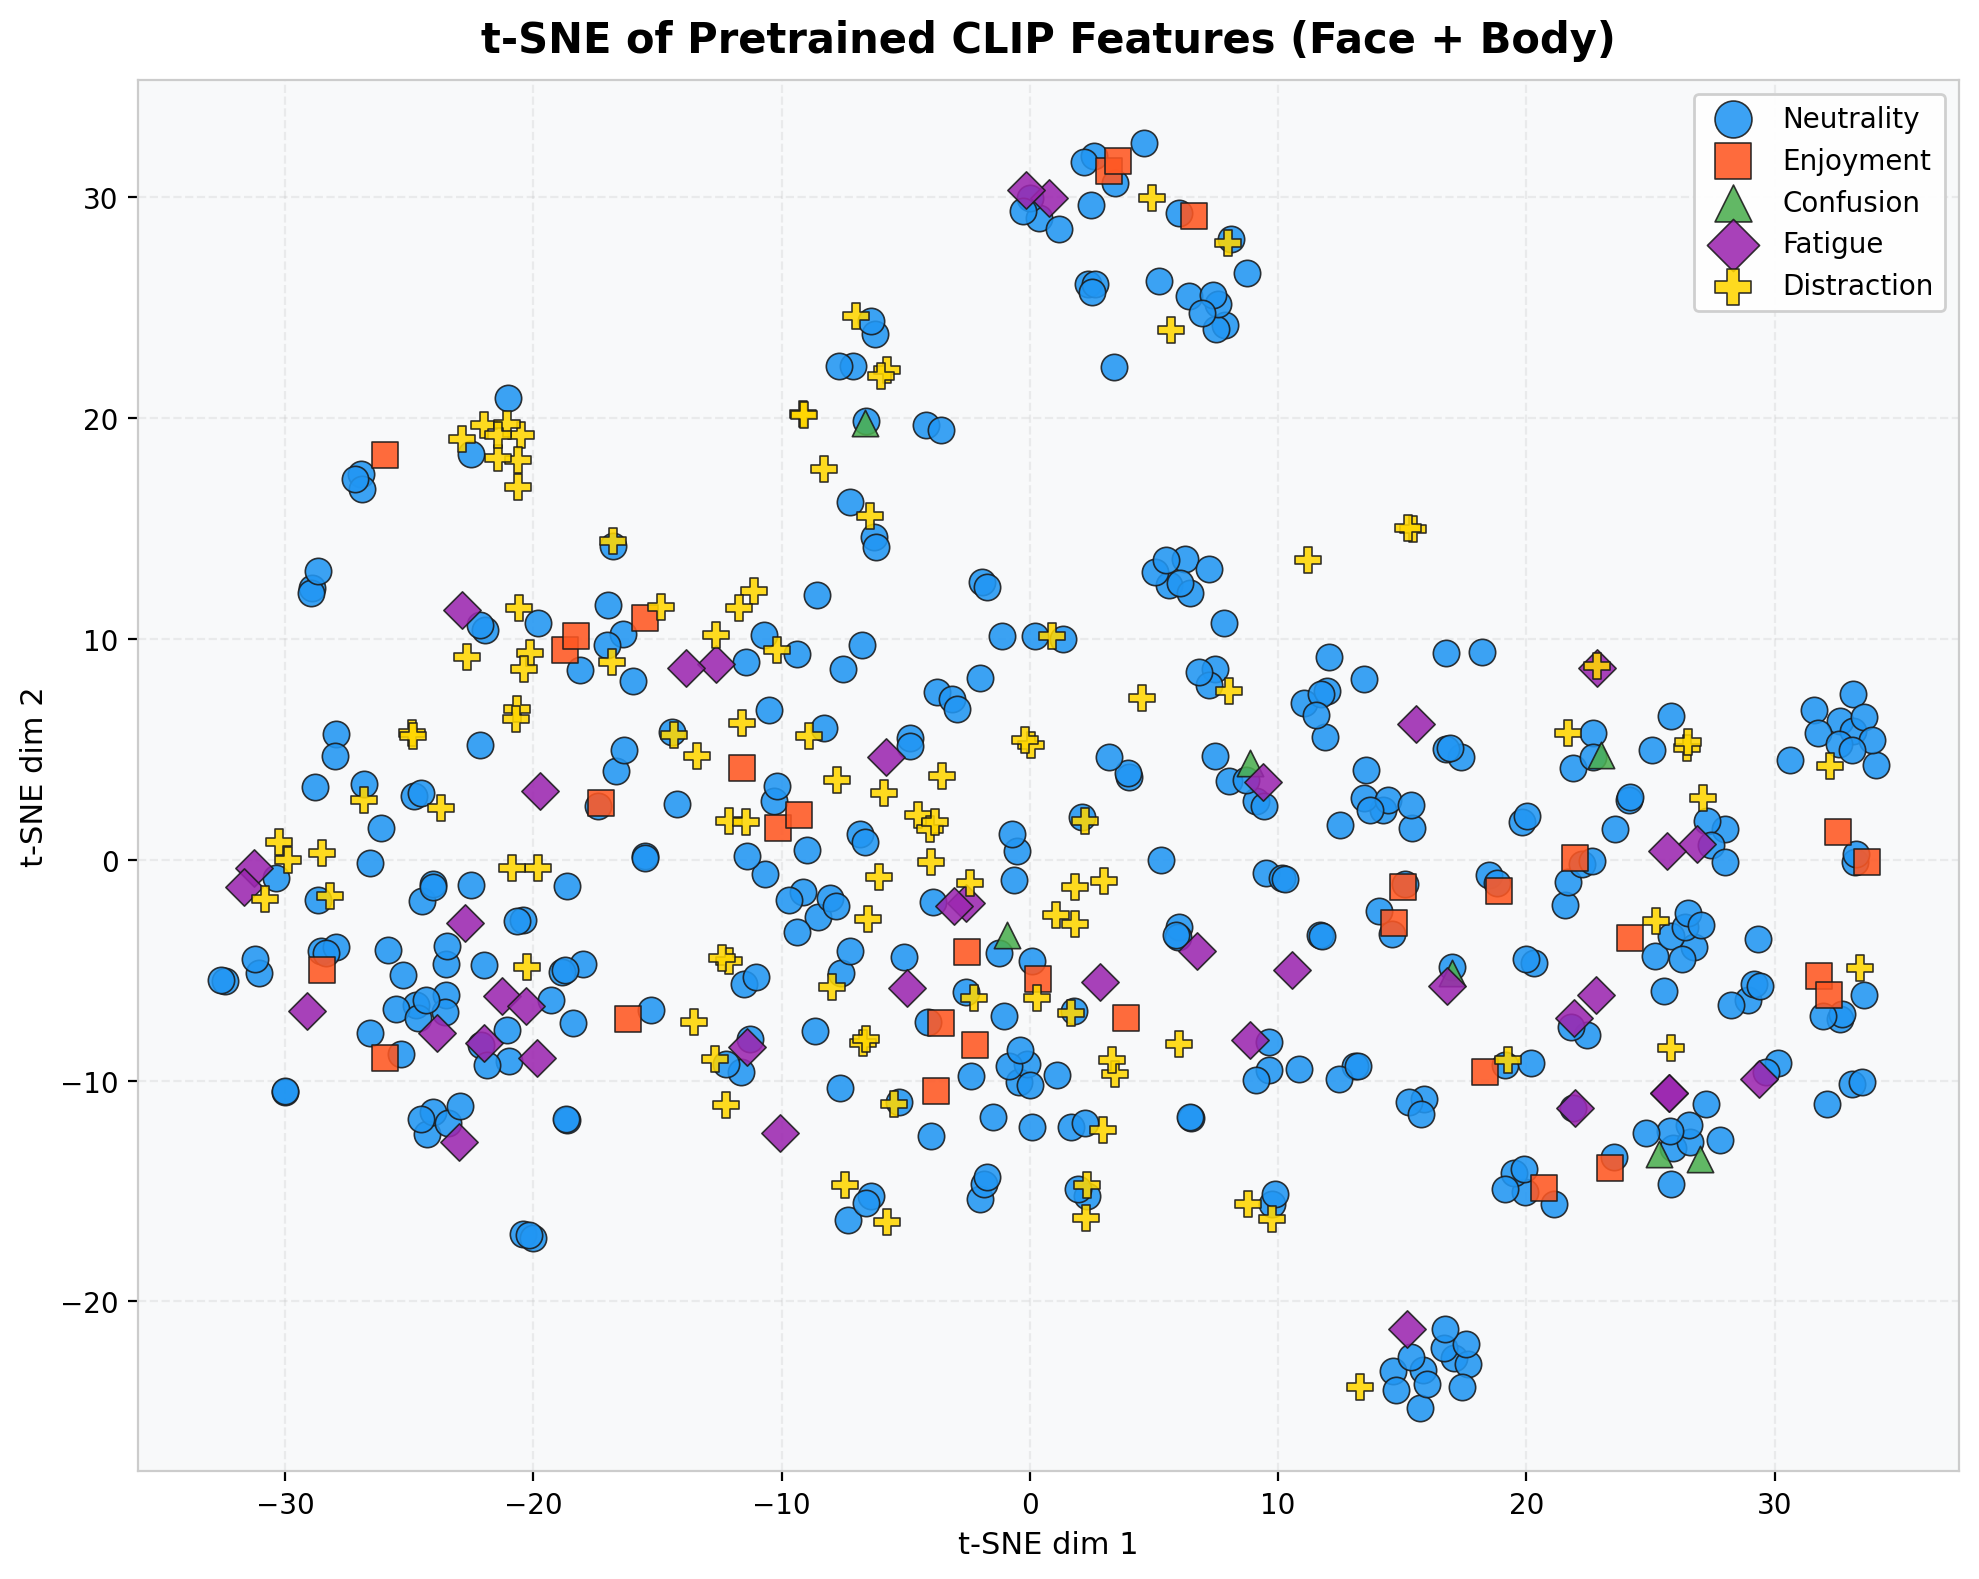
\includegraphics[width=\textwidth]{image/tsne_pretrained.png}
        \caption{Pretrained CLIP (Chưa fine-tune - Chồng lấn)}
        \label{fig:tsne_pre}
    \end{subfigure}
    \hfill
    \begin{subfigure}[b]{0.48\textwidth}
        \centering
        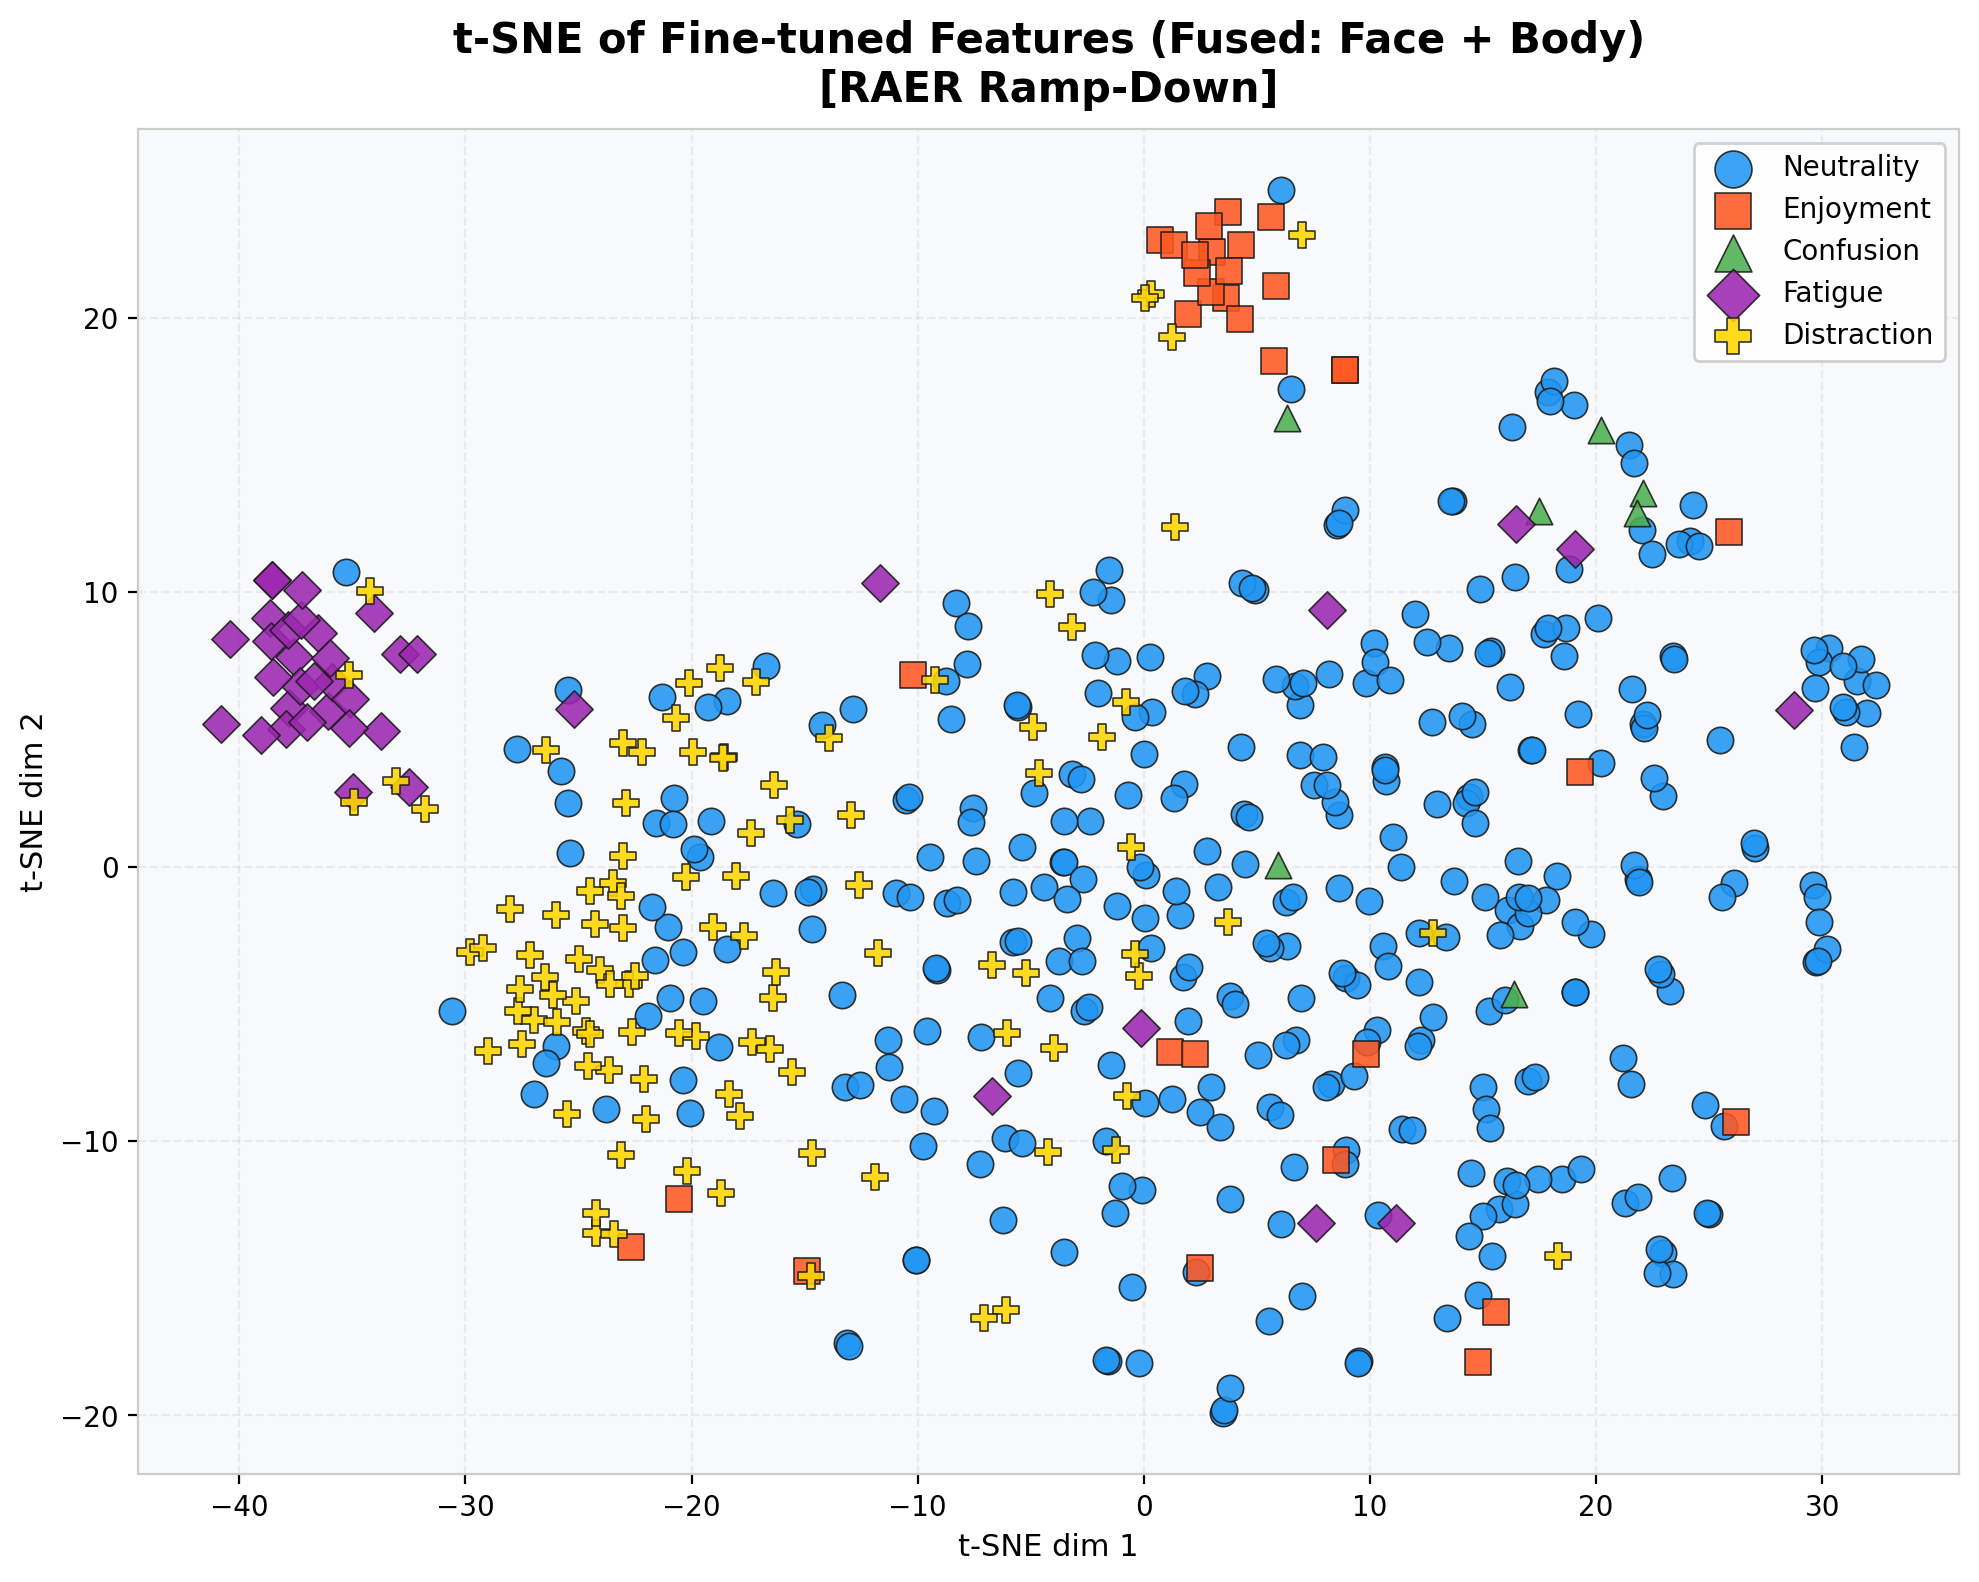
\includegraphics[width=\textwidth]{image/tsne_finetuned.png}
        \caption{RAPT-CLIP Đề xuất (Cụm tách biệt rõ rệt)}
        \label{fig:tsne_fine}
    \end{subfigure}
    \caption{So sánh không gian phân bố đặc trưng t-SNE trên 528 video kiểm thử RAER}
    \label{fig:tsne_comparison}
\end{figure}

\noindent\textbf{Nhận xét:} Với Pretrained CLIP, các mẫu cảm xúc bị phân tán hỗn loạn, biên phân lớp không rõ ràng, đặc biệt Neutrality, Confusion và Distraction bị trộn lẫn. Ngược lại, mô hình RAPT-CLIP Frame-Level Fusion sau khi tối ưu hóa qua CMAF và LDAM Loss giúp các vector đặc trưng co cụm chặt chẽ nội lớp (\textit{intra-class compact}) và tách biệt rõ rệt giữa các lớp (\textit{inter-class separable}).

\subsubsection{Đánh giá tính bền vững \& Khả năng chịu lỗi (Robustness - run\_robustness.py)}
Mô hình được kiểm tra trong các điều kiện khắc nghiệt ngoài thực tế để đo lường độ suy giảm hiệu năng:

\begin{table}[H]
\centering
\small
\caption{Đánh giá tính bền vững trước các dạng suy thoái dữ liệu trên tập kiểm thử RAER}
\label{tab:robustness}
\begin{tabularx}{\textwidth}{p{5.5cm} c c X}
\toprule
\rowcolor{tableheader}
\textbf{Điều kiện thử nghiệm} & \textbf{WAR (\%)} & \textbf{UAR (\%)} & \textbf{Mức suy giảm / Nhận xét} \\
\midrule
\rowcolor{grouprow} \multicolumn{4}{l}{\textbf{a. Che khuất luồng dữ liệu (Modality Occlusion)}} \\
\textbf{Gốc đầy đủ (Face + Body + Context)} & \textbf{77.65} & \textbf{77.06} & \textbf{Baseline tối ưu} \\
Che mất Context (Masked Context) & 79.55 & 68.58 & UAR giảm -8.48\% (Mất ngữ cảnh lớp hiếm) \\
Che mất Face (Masked Face) & 73.11 & 67.84 & \textbf{UAR giảm -9.22\%} (Mặt là luồng cốt lõi nhất) \\
Che mất Body (Masked Body) & 75.19 & 75.21 & UAR giảm nhẹ -1.85\% (Face + Context bù đắp) \\
\midrule
\rowcolor{grouprow} \multicolumn{4}{l}{\textbf{b. Bơm nhiễu thị giác Gaussian Noise ($\sigma$)}} \\
Nhiễu nhẹ ($\sigma = 0.1$) & 75.57 & 63.30 & Duy trì tốt 97\% WAR \\
Nhiễu vừa ($\sigma = 0.3$) & 61.17 & 41.79 & Suy giảm do mất các Action Units \\
Nhiễu nặng ($\sigma = 0.5$) & 32.01 & 24.47 & Mất thông tin thị giác nghiêm trọng \\
\midrule
\rowcolor{grouprow} \multicolumn{4}{l}{\textbf{c. Xáo trộn cấu trúc (Structural Disturbances)}} \\
\textbf{Xáo trộn thời gian (Temporal Shuffling)} & \textbf{77.46} & \textbf{74.28} & \textbf{Chỉ giảm -2.78\% UAR} (Attention Pooling bền vững) \\
Xóa ngẫu nhiên cơ thể (Random Erasing Body) & 76.70 & 71.66 & Chỉ giảm -5.40\% UAR \\
\bottomrule
\end{tabularx}
\end{table}

\begin{figure}[H]
    \centering
    \begin{subfigure}[b]{0.48\textwidth}
        \centering
        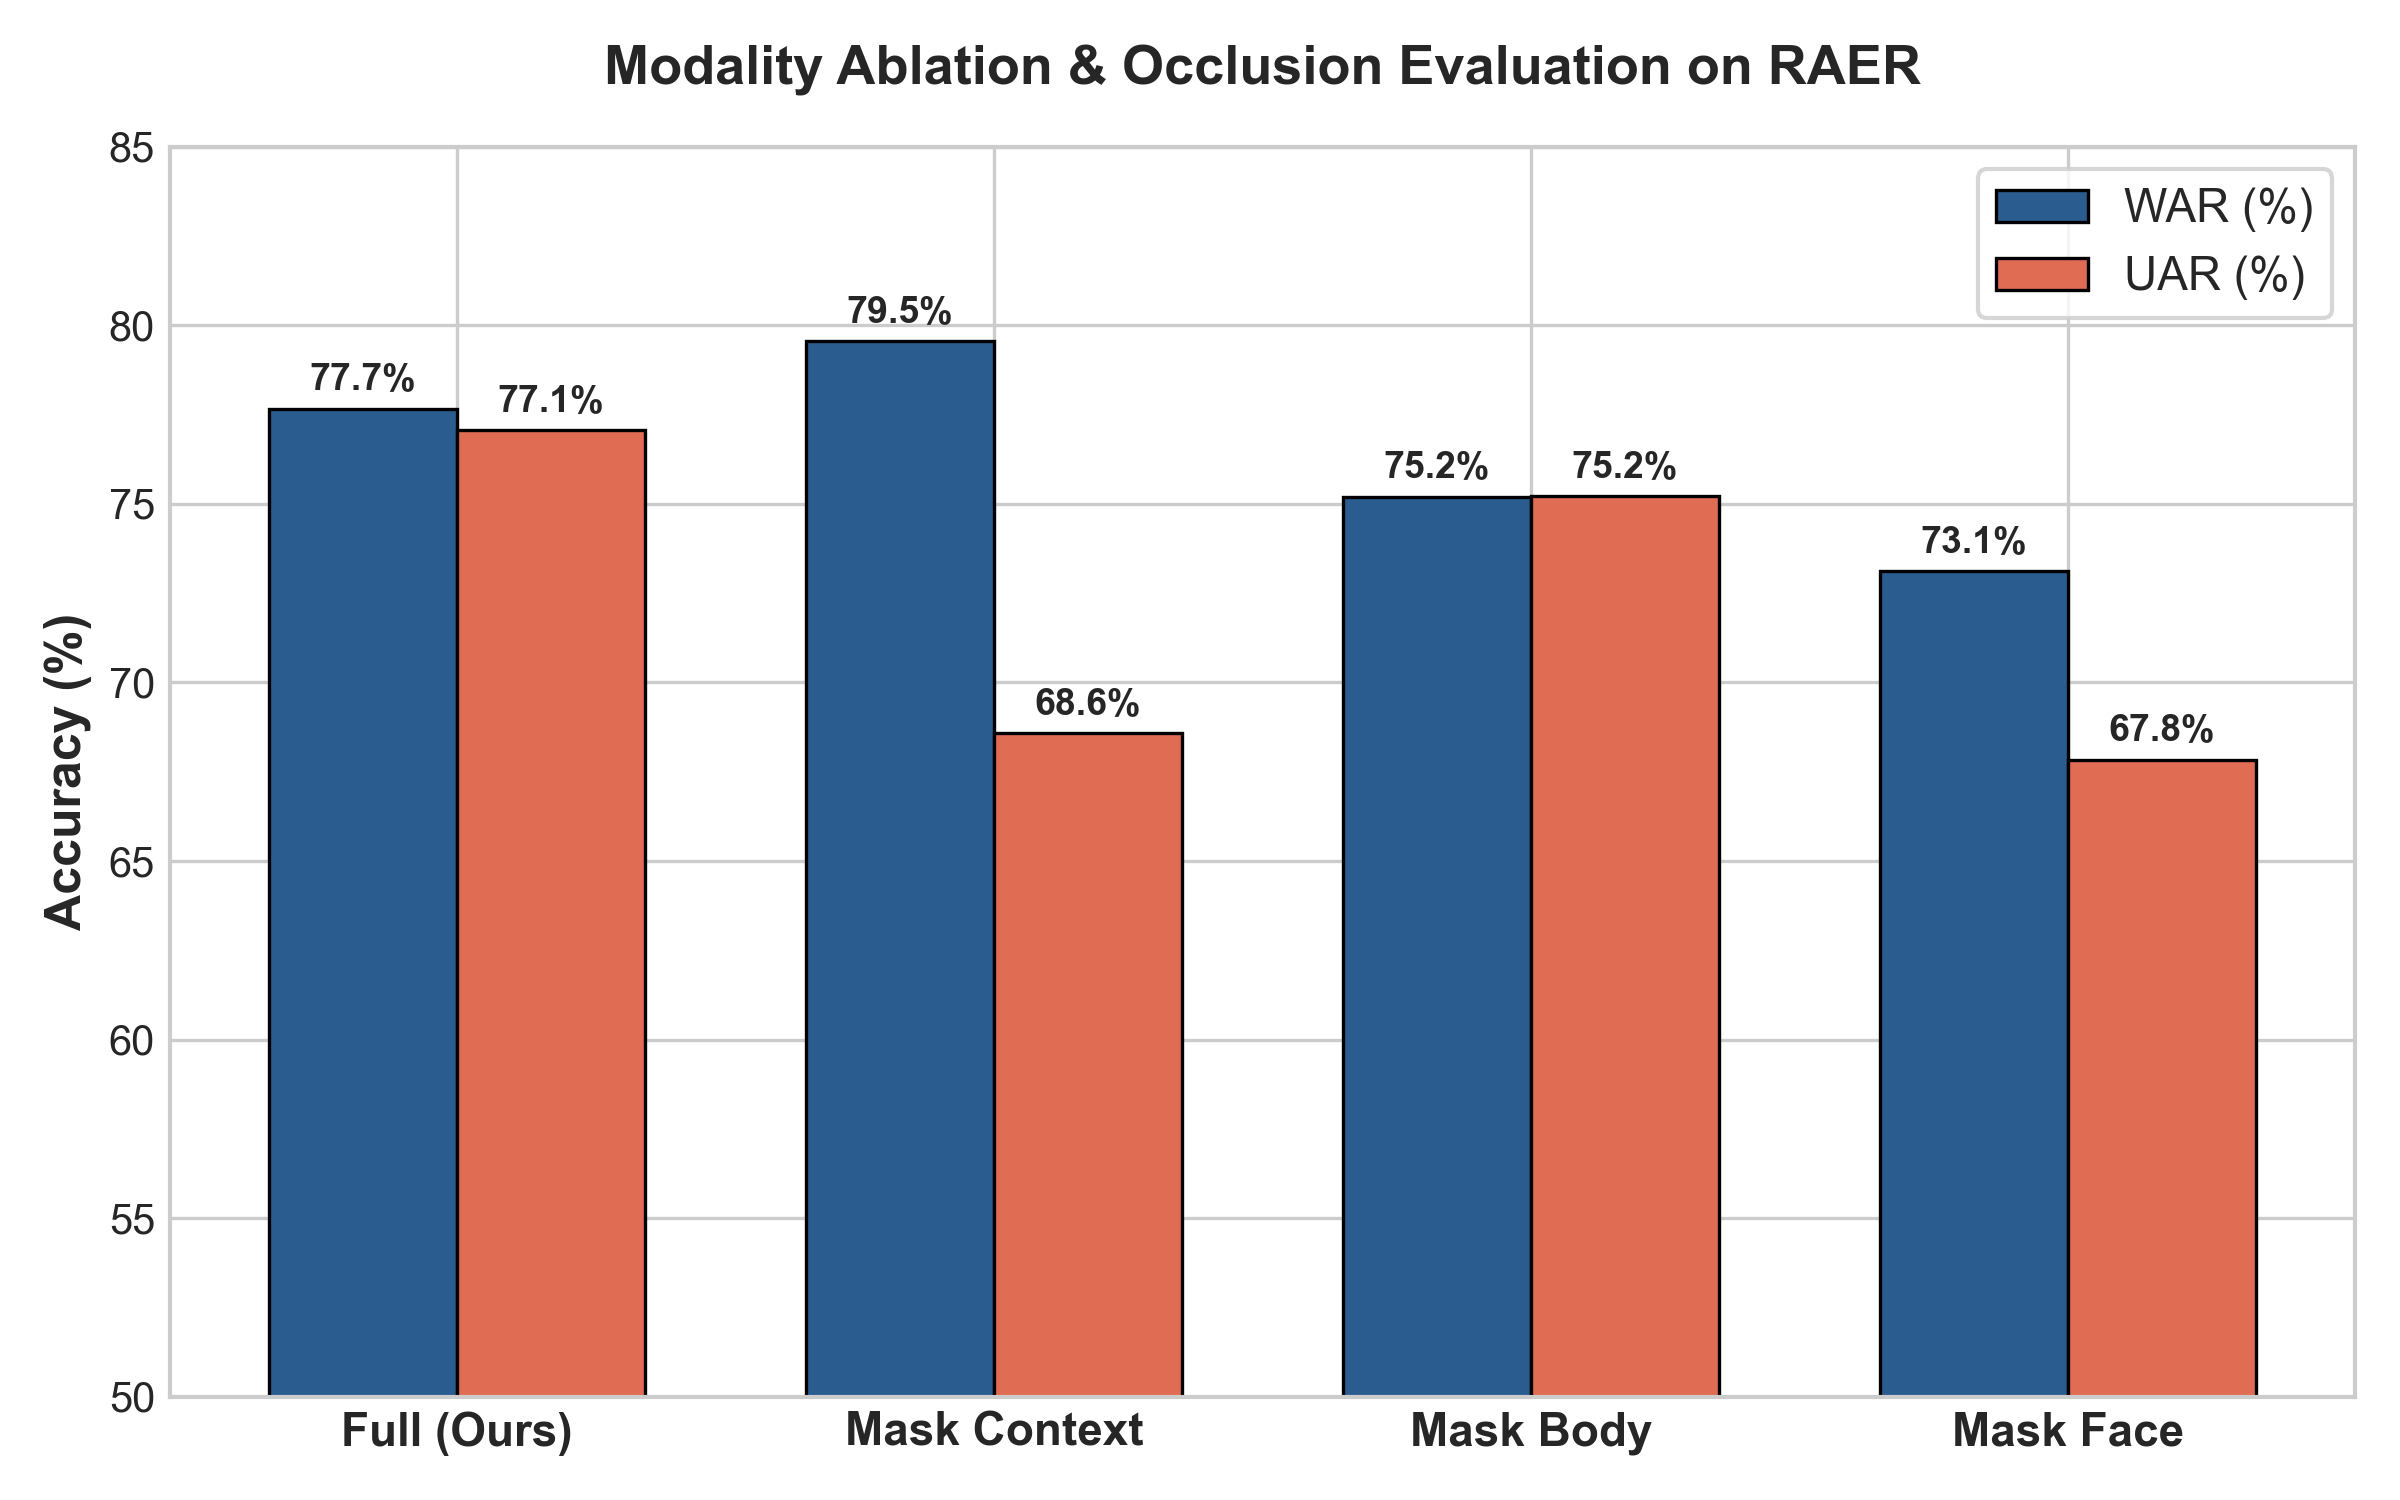
\includegraphics[width=\textwidth]{image/robustness_modality_ablation.png}
        \caption{Tác động khi che khuất từng luồng (Modality Occlusion)}
    \end{subfigure}
    \hfill
    \begin{subfigure}[b]{0.48\textwidth}
        \centering
        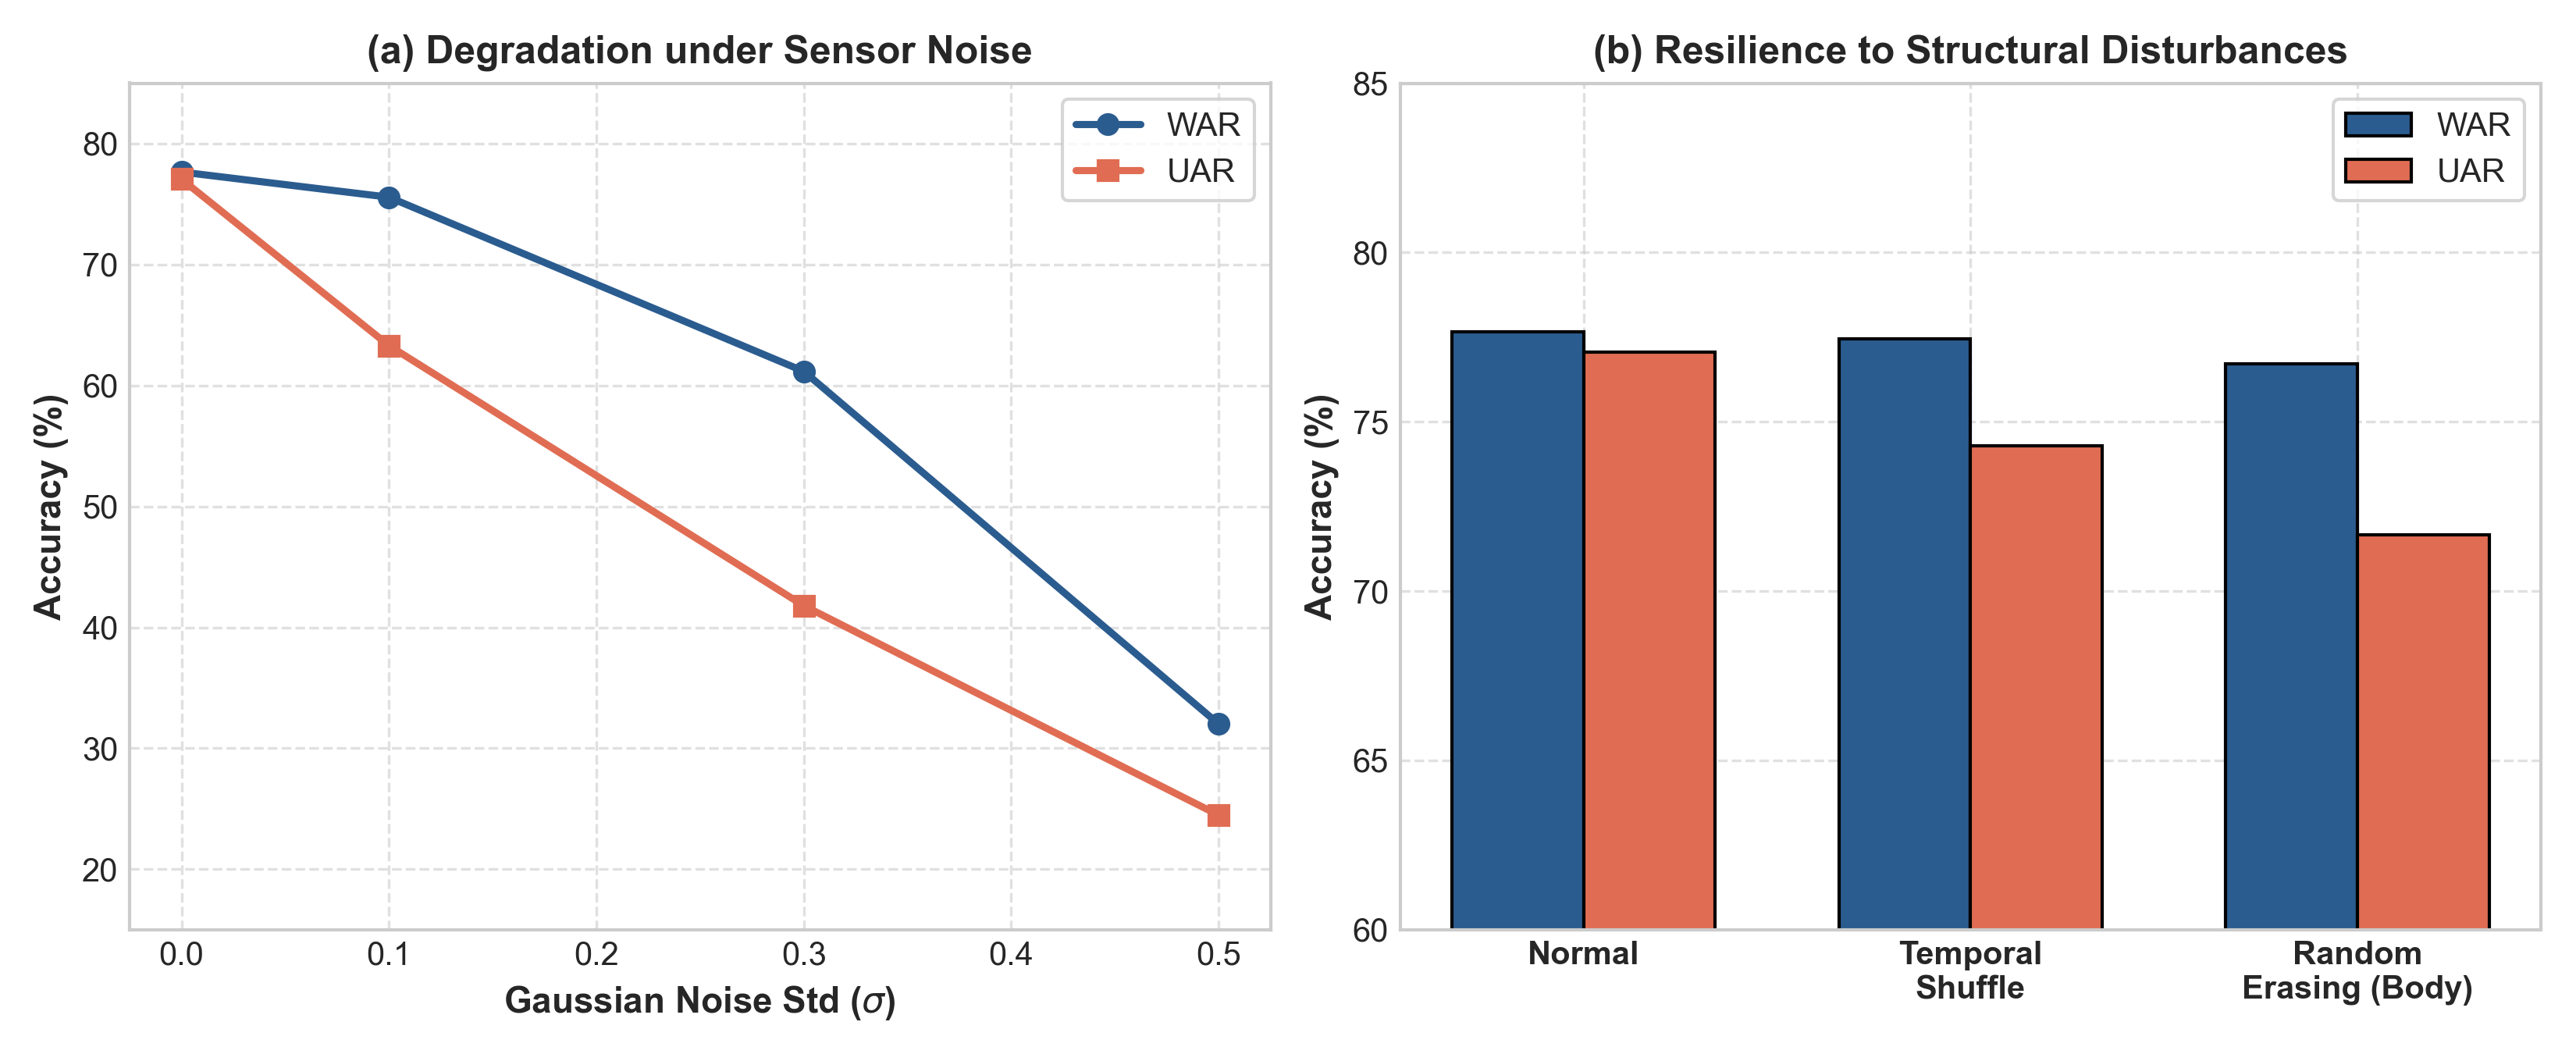
\includegraphics[width=\textwidth]{image/robustness_degradation.png}
        \caption{Đường cong suy giảm hiệu năng theo độ nhiễu Gaussian}
    \end{subfigure}
    \caption{Trực quan hóa độ bền vững của mô hình RAPT-CLIP}
    \label{fig:robustness_plots}
\end{figure}

\subsubsection{Đánh giá tính giải thích được với Grad-CAM (Interpretability)}
Bản đồ nhiệt kích hoạt Grad-CAM được trích xuất từ các khối Transformer block 8, 9, 10, 11 trên tập kiểm thử để xác định vùng mô hình tập trung quan sát:

\begin{figure}[H]
    \centering
    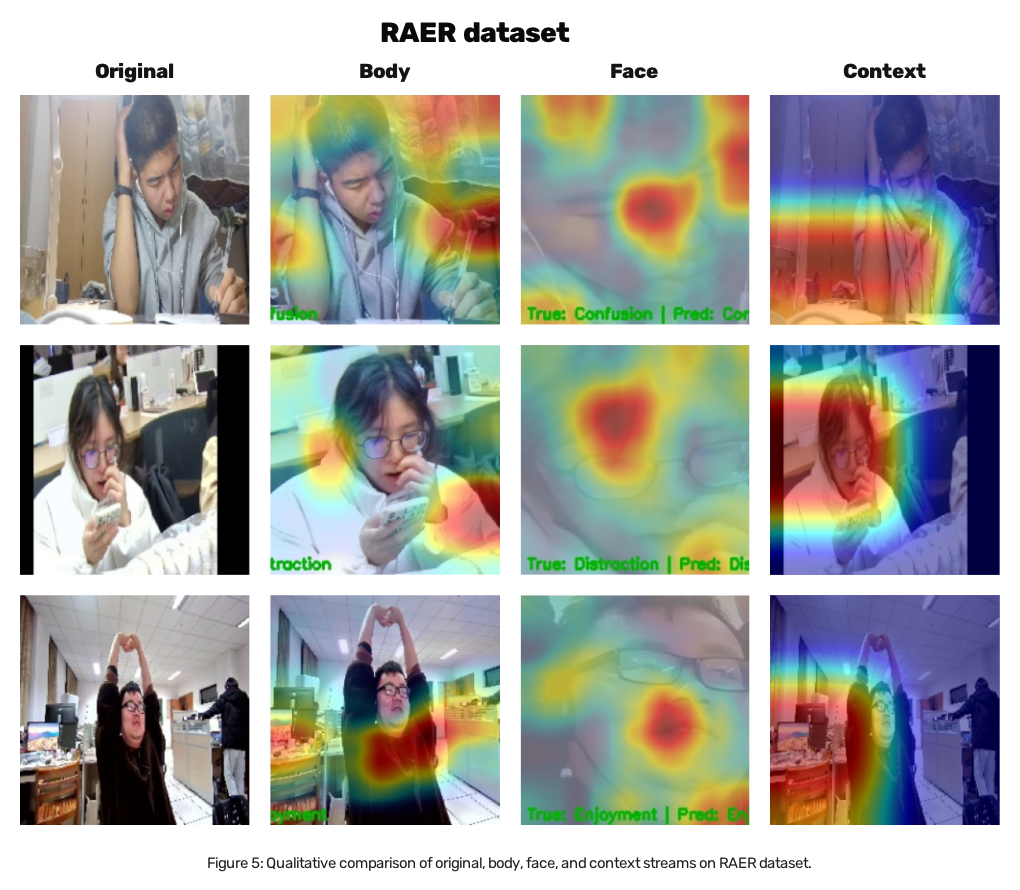
\includegraphics[width=0.95\textwidth, max height=7.5cm, keepaspectratio]{image/gradcam_sample.png}
    \caption{Trực quan hóa Grad-CAM 4 luồng [Gốc | Thân | Mặt | Bối cảnh]. Vùng nhiệt đỏ tập trung chính xác vào mắt, miệng trên Face và vai/tay trên Body.}
    \label{fig:gradcam_raer}
\end{figure}

% ==============================================================================
% MỤC 3: ABLATION STUDIES
% ==============================================================================
\section{Nghiên cứu cắt bỏ thành phần toàn diện (Ablation Studies)}

\noindent Nhằm định lượng giá trị đóng góp của từng module kiến trúc và phương pháp huấn luyện, các thử nghiệm cắt bỏ thành phần (\textit{Ablation Studies}) chuyên sâu đã được thực hiện trực tiếp trên tập kiểm thử chuẩn RAER (528 video), thể hiện chi tiết tại Bảng~\ref{tab:ablation}.

\begin{table}[H]
\centering
\small
\caption{Bảng tổng hợp kết quả Nghiên cứu cắt bỏ thành phần (Ablation Studies) trên RAER}
\label{tab:ablation}
\begin{tabularx}{\textwidth}{p{4.2cm} X c c p{3.2cm}}
\toprule
\rowcolor{tableheader}
\textbf{Biến thể mô hình} & \textbf{Cơ chế kiến trúc \& Kỹ thuật can thiệp} & \textbf{WAR} & \textbf{UAR} & \textbf{Chênh lệch / Đánh giá} \\
\midrule
\rowcolor{grouprow}
\textbf{RAPT-CLIP-FRAMELEVEL} & CMAF tại từng frame $\rightarrow$ Temporal Transformer $\rightarrow$ Concat Head + LDAM + Weighted Sampler + Loss MI/DC. & \textbf{77.65\%} & \textbf{77.06\%} & \textbf{Baseline tối ưu} (Cân bằng xuất sắc WAR \& UAR) \\
\addlinespace[2pt]
\textbf{RAPT-CLIP-VIDEOLEVEL} & \textbf{Sử dụng đủ 3 nhánh (Face+Body+Context)}, hoán đổi vị trí: Temporal từng nhánh riêng $\rightarrow$ CMAF mức Video $\rightarrow$ Concat Head. & {\color{accentred}\textbf{69.13\%}} & 76.64\% & \textbf{$\Delta$WAR: -8.52\%} (Mất đồng bộ vi mô giữa các luồng) \\
\addlinespace[2pt]
\texttt{RAER-no-weighted-sampler} & Dùng Random Sampler thông thường, không cân trọng số nhãn hiếm. & 84.09\% & {\color{accentred}\textbf{71.20\%}} & \textbf{$\Delta$UAR: -5.86\%} (Thiên vị đa số, bỏ rơi lớp hiếm) \\
\addlinespace[2pt]
\texttt{RAER-no-mi-dc} & Bỏ hàm tổn thất Thông tin tương hỗ ($\mathcal{L}_{\text{MI}}$) và Tương quan khoảng cách ($\mathcal{L}_{\text{DC}}$). & 79.73\% & {\color{accentred}\textbf{69.30\%}} & \textbf{$\Delta$UAR: -7.76\%} (Đặc trưng mặt và cảnh bị dư thừa) \\
\addlinespace[2pt]
\texttt{RAER-Freeze-image-encoder} & Đóng băng toàn bộ trọng số Visual Backbone CLIP ViT-B/16 (không fine-tune). & {\color{accentred}\textbf{58.33\%}} & 71.56\% & \textbf{$\Delta$WAR: -19.32\%} (Mất khả năng thích ứng cử chỉ) \\
\addlinespace[2pt]
\texttt{RAER-cross-entrophy} & Thay thế hàm tổn thất LDAM bằng Cross-Entropy tiêu chuẩn. & 79.73\% & {\color{accentred}\textbf{69.97\%}} & \textbf{$\Delta$UAR: -7.09\%} (Không mở rộng biên cho dữ liệu đuôi dài) \\
\addlinespace[2pt]
\texttt{RAER-drop-path} & Áp dụng ngắt đường truyền Stochastic Depth (Drop-Path) trong Transformer. & 73.30\% & {\color{accentred}\textbf{70.11\%}} & \textbf{$\Delta$UAR: -6.95\%} (Đứt gãy biểu cảm liên tục giữa các segment) \\
\bottomrule
\end{tabularx}
\end{table}

% ==============================================================================
% MỤC 4: BỘ DỮ LIỆU EMOTIC
% ==============================================================================
\section{Huấn luyện và Đánh giá trên bộ dữ liệu EMOTIC}

\noindent\textbf{Đặc điểm bộ dữ liệu:} EMOTIC là bộ dữ liệu cảm xúc ảnh tĩnh ngoài tự nhiên (\textit{Context-aware emotion recognition}) gồm 26 nhãn cảm xúc đa nhãn (\textit{Multi-label}) và 3 chiều cảm xúc liên tục VAD (\textit{Valence, Arousal, Dominance}).\\
\textbf{Cấu hình mô hình:} RAPT-CLIP sử dụng kiến trúc Triple-Stream (Face + Body + Context) dung hợp qua CMAF Frame-Level Fusion. Huấn luyện với hàm mất mát \textbf{Dynamic Asymmetric Loss (Dynamic ASL)} chuyên trị dữ liệu đa nhãn đuôi dài.\\
\textbf{Kết quả thực nghiệm chuẩn hóa (\texttt{model\_best.zip}):}
\begin{itemize}[leftmargin=18pt, itemsep=1pt]
    \item \textbf{Validation Macro mAP:} \textbf{46.98\%} (2,378 mẫu).
    \item \textbf{Test Macro mAP:} \textbf{34.76\%} (5,292 mẫu kiểm thử chính thức). Kết quả vượt trội so với baseline CVPR 2017 của Kosti et al. (27.38\% mAP, tăng \textbf{+7.38\%}) và mô hình EmotiCon CVPR 2020 (33.10\% mAP, tăng \textbf{+1.66\%}).
\end{itemize}

\subsection{Bảng siêu tham số huấn luyện chi tiết của bộ dữ liệu EMOTIC}

\begin{table}[H]
\centering
\small
\caption{Bảng siêu tham số huấn luyện chi tiết của mô hình RAPT-CLIP trên EMOTIC}
\label{tab:emotic_hyperparams}
\begin{tabularx}{\textwidth}{p{3.2cm} p{4.2cm} X}
\toprule
\rowcolor{tableheader}
\textbf{Nhóm tham số} & \textbf{Tên biến / Siêu tham số} & \textbf{Giá trị cấu hình thực nghiệm} \\
\midrule
\rowcolor{grouprow} \multicolumn{3}{l}{\textbf{a. Thiết lập huấn luyện chung \& Tối ưu hóa}} \\
Visual Backbone & \texttt{clip\_path}, \texttt{image\_size} & CLIP ViT-B/16 ($224 \times 224$), \texttt{freeze\_image\_encoder} = False \\
Epochs \& Batch Size & \texttt{epochs}, \texttt{batch\_size} & \textbf{25 Epochs} (Best: \textbf{Epoch 6}) $|$ Batch Size: \textbf{16} (Workers: 4) \\
Thuật toán tối ưu & \texttt{optimizer}, \texttt{weight\_decay} & \textbf{AdamW} $|$ Weight Decay: 0.005 $|$ Momentum: 0.9 $|$ Grad Clip: 1.0 \\
Tốc độ học (LRs) & \texttt{lr}, \texttt{lr\_image}, \texttt{lr\_prompt} & \texttt{lr}: \textbf{$1\times 10^{-4}$}, \texttt{lr\_image}: \textbf{$1\times 10^{-5}$}, \texttt{lr\_prompt}: \textbf{$5\times 10^{-5}$}, \texttt{lr\_adapter}: \textbf{$1\times 10^{-4}$} \\
Lịch điều phối LR & \texttt{scheduler}, \texttt{milestones} & MultiStepLR (Milestones: [10, 15], $\gamma = 0.1$, Warmup Epochs: 3) \\
\midrule
\rowcolor{grouprow} \multicolumn{3}{l}{\textbf{b. Hàm mất mát \& Xử lý mất cân bằng đa nhãn}} \\
Hàm mất mát chính & \texttt{loss\_type} (Dynamic ASL) & Dynamic Asymmetric Loss chuyên trị phân phối đa nhãn đuôi dài \\
Tham số ASL & \texttt{asl\_gamma\_neg}, \texttt{clip} & $\gamma_{-} = 4.0$, $\gamma_{+} = 0.0$, $\text{clip} = 0.05$ (Hạ áp lực gradient nhãn âm) \\
Hàm mất mát phụ & \texttt{lambda\_mi}, \texttt{lambda\_dc} & $\lambda_{\text{MI}} = 0.1$ (Warmup: 7, Ramp: 5), $\lambda_{\text{DC}} = 0.1$ (Warmup: 7, Ramp: 5) \\
Làm mượt nhãn & \texttt{label\_smoothing} & 0.05 (Giảm over-confidence trên các nhãn tần suất cao) \\
\midrule
\rowcolor{grouprow} \multicolumn{3}{l}{\textbf{c. Kiến trúc luồng \& Cơ chế suy luận}} \\
Luồng dữ liệu & \texttt{crop\_body}, \texttt{use\_context} & \textbf{Triple-Stream:} Face + Body + Context (Toàn cảnh nguyên bản) \\
Dung hợp đặc trưng & \texttt{fusion\_type}, \texttt{fusion\_stage} & \textbf{CMAF Frame-Level Fusion} (\texttt{stage=frame}, \texttt{modality\_dropout=0.3}) \\
Prompt Ensemble & \texttt{contexts\_number}, \texttt{text\_type} & Prompt Ensemble (8 contexts/lớp, \texttt{class\_specific\_contexts=True}) \\
Nhiệt độ \& Ngưỡng & \texttt{temperature}, \texttt{emotic\_threshold.json} & Temperature = 1.0 $|$ Ngưỡng quyết định tối ưu F1 quét trên tập Validation \\
\bottomrule
\end{tabularx}
\end{table}

\subsection{Trực quan hóa thứ bậc xếp hạng Test AP qua 26 cảm xúc}

\begin{figure}[H]
    \centering
    \includegraphics[width=0.95\textwidth, max height=7cm, keepaspectratio]{outputs/EMOTIC/emotic_test_ranking_barchart.png}
    \caption{Thứ bậc xếp hạng Test AP (\%) qua 26 nhãn cảm xúc EMOTIC (Đường gạch đứt đỏ: Macro mAP = 34.76\%)}
    \label{fig:emotic_bar}
\end{figure}

\subsection{Trực quan hóa Grad-CAM trên tập dữ liệu EMOTIC}
Bản đồ nhiệt kích hoạt Grad-CAM được trích xuất trực tiếp từ mô hình tối ưu (\texttt{model\_best.zip}) trên các mẫu kiểm thử EMOTIC:

\begin{figure}[H]
    \centering
    \begin{subfigure}[b]{0.32\textwidth}
        \centering
        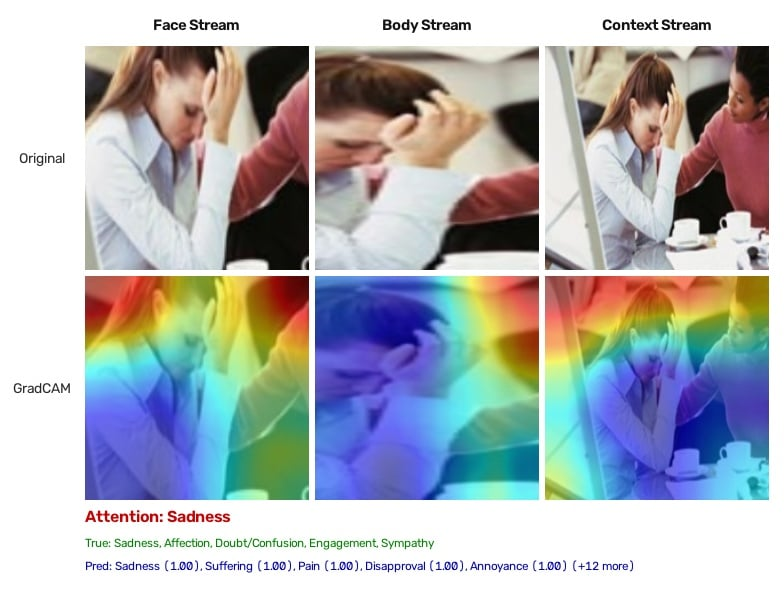
\includegraphics[width=\textwidth]{outputs/Gradcam-Emotic/1.jpeg}
        \caption{Mẫu 1: Tương tác mặt \& cảnh}
        \label{fig:emotic_grad_1}
    \end{subfigure}
    \hfill
    \begin{subfigure}[b]{0.32\textwidth}
        \centering
        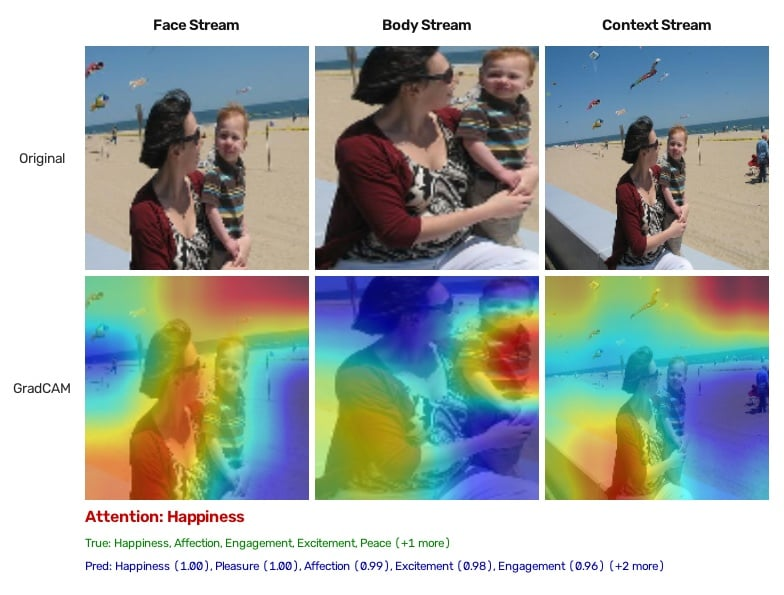
\includegraphics[width=\textwidth]{outputs/Gradcam-Emotic/2.jpeg}
        \caption{Mẫu 2: Cử chỉ hành vi cơ thể}
        \label{fig:emotic_grad_2}
    \end{subfigure}
    \hfill
    \begin{subfigure}[b]{0.32\textwidth}
        \centering
        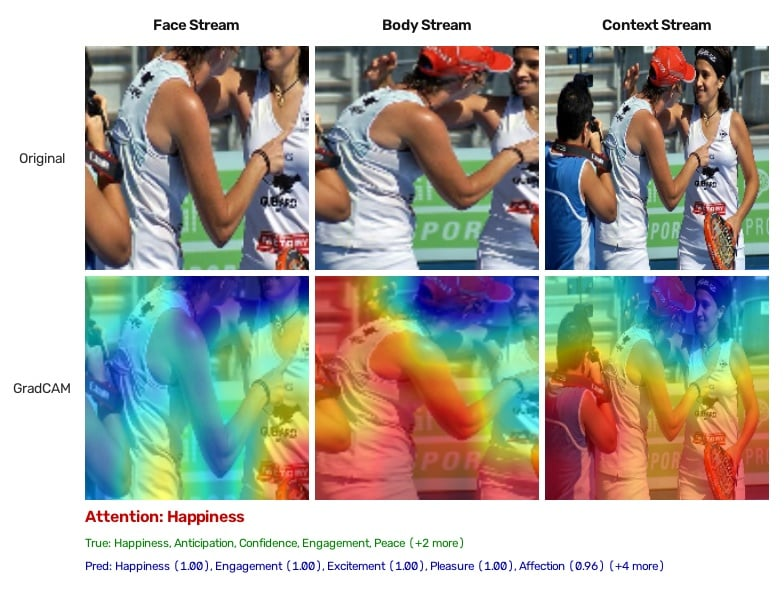
\includegraphics[width=\textwidth]{outputs/Gradcam-Emotic/3.jpeg}
        \caption{Mẫu 3: Cảm xúc phức hợp}
        \label{fig:emotic_grad_3}
    \end{subfigure}
    \caption{Trực quan hóa Grad-CAM trên tập dữ liệu EMOTIC (Thư mục: \texttt{outputs/Gradcam-Emotic/})}
    \label{fig:emotic_gradcam}
\end{figure}

\noindent\textbf{Nhận xét:} Các vùng nhiệt đỏ tập trung chính xác vào biểu cảm nét mặt và tư thế cơ thể người trong khung cảnh ngoài trời, chứng minh mô hình RAPT-CLIP đã dung hợp hài hòa cả 3 luồng thông tin (Face, Body, Context) để dự đoán chính xác cảm xúc ngoài ngữ cảnh tự nhiên.

% ==============================================================================
% MỤC 5: BỘ DỮ LIỆU CAER-S (STATIC)
% ==============================================================================
\section{Huấn luyện và Đánh giá trên bộ dữ liệu CAER-S (Static Images)}

\noindent\textbf{Đặc điểm bộ dữ liệu:} CAER-S (\textit{Context-Aware Emotion Recognition - Static}) là tập dữ liệu ảnh tĩnh quy mô lớn gồm 70,000 ảnh trích xuất từ 79 bộ phim truyền hình, bao gồm 7 lớp cảm xúc chuẩn: \textit{Anger, Disgust, Fear, Happy, Neutral, Sad, Surprise}. Tập huấn luyện gồm 49,007 ảnh với phân phối cân bằng hoàn hảo (đều đặn 7,001 mẫu/lớp), và tập kiểm định gồm 7,000 ảnh (1,000 mẫu/lớp).\\
\textbf{Cấu hình mô hình:} RAPT-CLIP sử dụng kiến trúc Triple-Stream (Face + Body + Masked Context) kết hợp cơ chế dung hợp \textbf{Tridirectional Frame-Level CMAF} (kích thước sau concat là 1536 chiều) và khối Temporal Transformer Attention Pooling (\texttt{temporal\_layers = 1}).\\
\textbf{Hàm mất mát \& Chiến lược tối ưu:} Mô hình áp dụng \textbf{LDAM Loss} ($s = 1.0, m_{\max} = 0.5$) kết hợp bộ lấy mẫu \textbf{WeightedRandomSampler}, điều phối tốc độ học \textbf{MultiStepLR} và kỹ thuật điều hòa đa mục tiêu \textbf{Mutual Information (MI: 0.1)} + \textbf{Decorrelation (DC: 0.1)}.\\
\textbf{Kết quả thực nghiệm vượt bậc (Đạt đỉnh tại Epoch 19):}
\begin{itemize}[leftmargin=18pt, itemsep=1pt]
    \item \textbf{Train WAR / UAR:} \textbf{96.55\%} (Loss: 0.5419).
    \item \textbf{Validation WAR (Overall Accuracy):} \textbf{90.40\%} (6,328 / 7,000 mẫu chính xác, Loss: 0.6787).
    \item \textbf{Validation UAR (Balanced Accuracy):} \textbf{90.40\%} $|$ \textbf{Harmonic Score:} \textbf{90.40\%}.
    \item \textbf{So sánh với các SOTA thế giới:} Vượt qua hàng loạt mô hình hàng đầu như MA-Net (88.42\%) và GLAMOR-Net (89.88\%), áp sát AGCD-Net (90.65\%) và SAFER (91.40\%).
\end{itemize}

\subsection{Bảng siêu tham số huấn luyện của bộ dữ liệu CAER-S}

\begin{table}[H]
\centering
\small
\caption{Bảng siêu tham số huấn luyện chi tiết của mô hình RAPT-CLIP trên CAER-S (Script: \texttt{caer\_s\_cmaf.sh})}
\label{tab:caers_hyperparams}
\begin{tabularx}{\textwidth}{p{3.2cm} p{4.2cm} X}
\toprule
\rowcolor{tableheader}
\textbf{Nhóm tham số} & \textbf{Tên biến / Siêu tham số} & \textbf{Giá trị cấu hình thực nghiệm} \\
\midrule
\rowcolor{grouprow} \multicolumn{3}{l}{\textbf{a. Thiết lập huấn luyện \& Tối ưu hóa}} \\
Visual Backbone & \texttt{clip\_path}, \texttt{image\_size} & CLIP ViT-B/16 ($224 \times 224$), \texttt{freeze\_image\_encoder} = False \\
Epochs \& Batch Size & \texttt{epochs}, \texttt{batch\_size} & \textbf{20 Epochs} (Đạt đỉnh: \textbf{Epoch 19}) $|$ Batch Size: \textbf{16} (Workers: 4) \\
Thuật toán tối ưu & \texttt{optimizer}, \texttt{weight\_decay} & \textbf{AdamW} $|$ Weight Decay: 0.005 $|$ Momentum: 0.9 $|$ Grad Clip: 1.0 \\
Tốc độ học (LRs) & \texttt{lr}, \texttt{lr\_image}, \texttt{lr\_prompt} & \texttt{lr}: \textbf{$2\times 10^{-5}$}, \texttt{lr\_image}: \textbf{$1\times 10^{-6}$}, \texttt{lr\_prompt}: \textbf{$3\times 10^{-4}$}, \texttt{lr\_adapter}: \textbf{$1\times 10^{-4}$} \\
Lịch điều phối LR & \texttt{scheduler}, \texttt{milestones} & \textbf{MultiStepLR} (Milestones: [10, 15], $\gamma = 0.1$) \\
\midrule
\rowcolor{grouprow} \multicolumn{3}{l}{\textbf{b. Hàm mất mát \& Điều hòa biểu diễn}} \\
Hàm mất mát chính & \texttt{loss\_type}, \texttt{ldam\_s}, \texttt{max\_m} & \textbf{LDAM Loss} (\texttt{loss\_type = ldam}, $s = 1.0$, $m_{\max} = 0.5$) \\
Bộ lấy mẫu & \texttt{use\_weighted\_sampler} & \textbf{WeightedRandomSampler} (Cân bằng phân phối mini-batch) \\
Làm mượt nhãn & \texttt{label\_smoothing} & 0.05 (Hạn chế hiện tượng over-confidence) \\
Hàm mất mát phụ & \texttt{lambda\_mi}, \texttt{lambda\_dc} & $\lambda_{\text{MI}} = 0.1$ (Warmup: 3, Ramp: 6), $\lambda_{\text{DC}} = 0.1$ (Warmup: 3, Ramp: 6) \\
Regularization & \texttt{drop\_path\_rate}, \texttt{modality\_dropout} & DropPath: 0.0 $|$ Modality Dropout: 0.0 \\
\midrule
\rowcolor{grouprow} \multicolumn{3}{l}{\textbf{c. Luồng dữ liệu \& Kiến trúc dung hợp}} \\
Luồng dữ liệu & \texttt{crop\_body}, \texttt{mask\_context\_face} & \textbf{Triple-Stream:} Face Crop + Body Crop (Torso) + Context (Xóa mặt) \\
Dung hợp đặc trưng & \texttt{fusion\_type}, \texttt{fusion\_stage} & \textbf{Tridirectional Frame-Level CMAF} (1536-d) $|$ Temporal Layers: 1 (\texttt{attn}) \\
Prompt Ensemble & \texttt{contexts\_number}, \texttt{text\_type} & Prompt Ensemble (8 learnable context tokens/lớp, CoOp tuning) \\
Nhiệt độ & \texttt{temperature} & $\tau = 0.07$ (Chuẩn cosine similarity của CLIP) \\
\bottomrule
\end{tabularx}
\end{table}

\subsection{So sánh với các phương pháp SOTA trên CAER-S}

\begin{table}[H]
\centering
\small
\caption{So sánh hiệu năng nhận diện cảm xúc của RAPT-CLIP với các phương pháp SOTA trên CAER-S}
\label{tab:caers_sota_comparison}
\begin{tabularx}{\textwidth}{l l c c X}
\toprule
\rowcolor{tableheader}
\textbf{Phương pháp} & \textbf{Nguồn / Năm} & \textbf{WAR (\%)} & \textbf{UAR (\%)} & \textbf{Đặc trưng kiến trúc chính} \\
\midrule
CAER-Net-S & Lee et al., ICCV 2019 & 73.51 & 73.51 & 2-Stream CNN (Face + Context) \\
EmotiCon & Mittal et al., AAAI 2020 & 77.00 & 77.00 & Đa nhánh: Mặt, Dáng, Cảnh, Độ sâu \\
GRERN & 2021 & 81.31 & 81.31 & Đồ thị quan hệ ngữ cảnh \\
EfficientFace & 2021 & 85.87 & 85.87 & Mạng khuôn mặt nhẹ hiệu năng cao \\
MA-Net & 2021 & 88.42 & 88.42 & Chú ý đa góc nhìn khuôn mặt \& bối cảnh \\
GLAMOR-Net & 2023 & 89.88 & 89.88 & Tương tác toàn cục và cục bộ \\
AGCD-Net & 2023 & 90.65 & 90.65 & Phân tách đồ thị thích ứng \\
SAFER & 2024 & 91.40 & 91.40 & Tinh chỉnh ngữ cảnh nâng cao \\
\midrule
\rowcolor{grouprow}
\textbf{RAPT-CLIP (Ours)} & \textbf{Công trình này (Epoch 19)} & \textbf{90.40} & \textbf{90.40} & \textbf{Triple-Stream CMAF + CLIP + LDAM Loss ($s=1.0$)} \\
\bottomrule
\end{tabularx}
\end{table}

\subsection{Phân tích độ hồi tưởng (Recall) chi tiết từng lớp cảm xúc \& Ma trận nhầm lẫn}

\noindent Dưới đây là bảng phân tích chi tiết tỷ lệ nhận diện chính xác trên từng lớp cảm xúc tại Epoch 7:

\begin{table}[H]
\centering
\small
\caption{Độ hồi tưởng (Recall) trên từng lớp cảm xúc của tập kiểm định CAER-S (1,000 mẫu/lớp)}
\label{tab:caers_per_class}
\begin{tabularx}{\textwidth}{c l c c X}
\toprule
\rowcolor{tableheader}
\textbf{ID} & \textbf{Nhãn cảm xúc} & \textbf{Số mẫu đúng / 1,000} & \textbf{Recall (\%)} & \textbf{Nhận xét đặc trưng nhận diện} \\
\midrule
0 & \textbf{Anger} & 923 / 1000 & \textbf{92.30\%} & Nhận diện xuất sắc qua biểu cảm cau mày và tư thế giận dữ \\
1 & \textbf{Disgust} & 981 / 1000 & \textbf{98.10\%} & Gần như hoàn hảo; nhăn mũi và né tránh bối cảnh \\
2 & \textbf{Fear} & 997 / 1000 & \textbf{99.70\%} & Cực kỳ vượt trội (chỉ nhầm 3 mẫu); mắt mở to và co người \\
3 & \textbf{Happy} & 834 / 1000 & \textbf{83.40\%} & Nụ cười và ánh mắt sáng; đôi lúc nhầm sang Neutral (70 mẫu) \\
4 & \textbf{Neutral} & 737 / 1000 & \textbf{73.70\%} & Lớp khó nhất; phân tán nhẹ sang Surprise (68) và Happy (56) \\
5 & \textbf{Sad} & 934 / 1000 & \textbf{93.40\%} & Khóe môi trễ xuống và dáng người buông thõng thể hiện rõ \\
6 & \textbf{Surprise} & 922 / 1000 & \textbf{92.20\%} & Mắt trợn tròn và há miệng được CMAF bắt trúng \\
\midrule
\rowcolor{grouprow}
\multicolumn{2}{l}{\textbf{Trung bình toàn bộ (WAR / UAR)}} & \textbf{6,328 / 7,000} & \textbf{90.40\%} & \textbf{Hiệu năng đồng đều vượt trội trên cả 7 cảm xúc} \\
\bottomrule
\end{tabularx}
\end{table}

\begin{table}[H]
\centering
\small
\caption{Ma trận nhầm lẫn thực nghiệm trên tập kiểm định CAER-S tại Epoch 7 (7,000 mẫu)}
\label{tab:caers_cm}
\begin{tabular}{r | rrrrrrr | r}
\toprule
\rowcolor{tableheader}
\textbf{True $\backslash$ Pred} & \textbf{Anger} & \textbf{Disgust} & \textbf{Fear} & \textbf{Happy} & \textbf{Neutral} & \textbf{Sad} & \textbf{Surprise} & \textbf{Tổng} \\
\midrule
\textbf{Anger}    & \textbf{923} & 10  & 1   & 7   & 28  & 17  & 14  & 1,000 \\
\textbf{Disgust}  & 4   & \textbf{981} & 2   & 4   & 1   & 7   & 1   & 1,000 \\
\textbf{Fear}     & 0   & 1   & \textbf{997} & 0   & 0   & 2   & 0   & 1,000 \\
\textbf{Happy}    & 25  & 4   & 8   & \textbf{834} & 70  & 17  & 42  & 1,000 \\
\textbf{Neutral}  & 53  & 29  & 10  & 56  & \textbf{737} & 47  & 68  & 1,000 \\
\textbf{Sad}      & 16  & 1   & 5   & 11  & 19  & \textbf{934} & 14  & 1,000 \\
\textbf{Surprise} & 19  & 3   & 3   & 16  & 22  & 15  & \textbf{922} & 1,000 \\
\bottomrule
\end{tabular}
\end{table}

% ==============================================================================
% MỤC 6: BỘ DỮ LIỆU CAER (VIDEO)
% ==============================================================================
\section{Huấn luyện trên bộ dữ liệu CAER Video}
\begin{itemize}[leftmargin=18pt, itemsep=2pt]
    \item \textbf{Đặc điểm bộ dữ liệu:} Bộ dữ liệu cảm xúc trích từ các video phim truyền hình (\textit{Context-Aware Emotion Recognition}) gồm 7 lớp cảm xúc cơ bản.
    \item \textbf{Cấu hình huấn luyện:} Tập lệnh thực thi \texttt{train\_sh/caer\_cmaf.sh}. Tải trước đặc trưng CLIP dưới dạng file \texttt{.npy} để tối ưu hóa tốc độ I/O. Dung hợp 2 luồng Face và Context qua CMAF (kích thước sau concat là 1024 chiều), sau đó ánh xạ qua Projection Head để phân loại cảm xúc.
\end{itemize}

\section{Huấn luyện trên bộ dữ liệu DAISEE}
\begin{itemize}[leftmargin=18pt, itemsep=2pt]
    \item \textbf{Đặc điểm bộ dữ liệu:} Bộ dữ liệu video đánh giá mức độ tập trung học tập trực tuyến (\textit{Academic Engagement Dataset}) gồm 4 trạng thái: Engagement, Boredom, Confusion, Frustration.
    \item \textbf{Cấu hình huấn luyện:} Tập lệnh thực thi \texttt{train\_sh/daisee\_cmaf.sh}. Lấy mẫu 16 segments video, tích hợp thuật toán OpenCV YuNet để tự động crop khuôn mặt chuẩn xác từ epoch đầu tiên. Kết hợp Prompt Ensemble chuyên biệt về hướng mắt và sự tập trung, huấn luyện với hàm mất mát LDAM và Weighted Sampler nhằm khắc phục triệt để hiện tượng mất cân bằng lớp trầm trọng.
\end{itemize}

\end{document}
